% !TEX root = saveliev_physics_general_course_1.tex
%!TEX TS-program = pdflatex
%!TEX encoding = UTF-8 Unicode


\chapter{CHUYỂN ĐỘNG DAO ĐỘNG}\label{chap:7}

\section{Các kiến thức chung về dao động}\label{sec:7_1}

Người ta gọi các quá trình có đặc tính lặp lại ở một mức độ nào đó là các dao động. Chẳng hạn, sự đu đưa của con lắc đồng hồ, dao động của sợi dây hoặc của nhánh âm thoa, hiệu điện thế giữa hai bản tụ điện trong mạng rađiô, v.v… đều có tính chất lặp lại như vậy.

Người ta phân biệt các dao động tùy theo bản chất vật lý của quá trình lặp lại: các dao động cơ, điện từ, điện cơ, v.v… Trong chương này ta nghiên cứu các dao động cơ.

Các dao động thường gặp một cách phổ biến trong tự nhiên và kỹ thuật. Trong nhiều trường hợp chúng có vai trò tiêu cực. Các dao động của cầu xuất hiện do các va đập mà bánh xe tàu hỏa truyền cho cầu khi đi quá các chỗ nối các đường ray, các dao động (các rung động) của thân tàu thủy gây ra bởi sự quay của chân vịt, các rung động của cánh máy bay — tất cả các quá trình đó dẫn tới các kết quả tai hại. Trong các trường hợp như thế vấn đề là ở chỗ làm thế nào để ngăn ngừa sự xuất hiện các dao động hoặc, trong mọi trường hợp, ngăn cản các dao động đạt tới các mức độ nguy hiểm.
Đồng thời các quá trình dao động sẽ là cơ sở của các lĩnh vực kỹ thuật khác nhau. Chẳng hạn, toàn bộ kỹ thuật vô tuyến điện dựa trên các quá trình dao động. Tùy thuộc vào tính chất của tác đông lên hệ dao động người ta phân biệt các dao động tự do (hoặc các dao động riêng), các dao động cưỡng bức, các tự dao động và các dao động tham số.

Các \textbf{dao động tự do} hoặc các \textbf{dao động riêng} là các dao động xảy ra trong một hệ được tự do sau khi truyền cho hệ một sự va đập hoặc là sau khi hệ được đưa ra khỏi vị trí cân bằng. Để làm ví dụcó thể lấy dao động của một quả cầu treo vào một sợi dây (con lắc). Để gây ra dao động có thể hoặc va đập vào quả cầu hoặc đẩy nó về một bên rồi buông ra.

Các \textbf{dao động cưỡng bức} là các dao động mà trong quá trình dao động hệ dao động chịu tác động các ngoại lực biến đổi tuần hoàn. Để làm ví dụ người ta dùng dao động của cầu xuất hiện khi đoàn người diễu hành qua nó.

Các \textbf{tự dao động}, cũng như các dao động cưỡng bức, xảy ra cùng với tác động của các ngoại lực lên hệ dao động, tuy nhiên các thời điểm mà các tác động này được thực hiện sẽ được quy định bởi chính hệ dao động, nghĩa là hệ điều khiển tác động bên ngoài. Làm ví dụ cho hệ tự dao động là đồng hồ, trong đó con lắc nhận được các va đập do năng lượng của một quả cân được nâng lên hoặc của một lò xo bị xoắn, thêm đó các va đập này xảy ra vào những lúc con lắc đi qua vị trí trung bình..

Trong các \textbf{dao động tham số} thì sự biến đổi tuần hoàn của một tham số nào đó của hệ sẽ xảy ra do tác động bên ngoài, chẳng hạn, của độ dài sợi dây treo quả cầu thực hiện dao động

Các dao động đơn giản nhất là các \textbf{Dao động điều hòa}, nghĩa là các dao động trong đó đại lượng dao động (chẳng hạn, độ lệch của con lắc) biến đổi với thời gian theo định luật $\sin$ hay $\cos$. Dạng dao động này là đặc biệt quan trọng vì các lý do sau đây; trước hết, các dao động trong tự nhiên và trong kỹ thuật thường có tính chất rất gần với dao động điều hòa và thứ hai, các quá trình tuần hoàn có dạng khác (với sự phụ thuộc khác vào thời gian) có thể được biểu diễn như sự chồng một số dao động điều hòa.

\section{Các dao động bé}\label{sec:7_2}

Ta xét một hệ cơ học có vị trí có thể được cho bởi một đại lượng mà ta ký hiệu là $x$. Trong những trường hợp như vậy người ta nói rằng hệ có một bậc tự do. Đại lượng $x$ xác định vị trí của hệ có thể là góc tính từ một mặt phẳng nào đó hoặc khoảng cách tính dọc theo đường cong đã cho (nói riêng là đường thẳng), v.v... Thế năng của hệ sẽ là hàm của một biến $x$: $E_{\text{p}}=E_{\text{p}}(x)$. Giả thử hệ có một vị trí cân bằng bền. Tại vị trí này hàm $U(x)$ có cực tiểu [Xem mục \S~\ref{sec:3_9}]. Ta quy ước tính tọa độ $x$ và thế năng $E_{\text{p}}$ từ vị trí cân bằng. Khi đó $E_{\text{p}}(0)=0$.

Phân tích hàm $E_{\text{p}}(x)$ thành chuỗi theo lũy thừa của $x$, thêm vào đó hạn chế bằng việc xét các dao động bé, cho nên có thể sẽ bỏ qua các lũy thừa bậc cao của $x$. Theo công thức Mac Laurent
\begin{equation*}
	E_{\text{p}}(x) = E_{\text{p}}(0) + E_{\text{p}}'(0)\,x + \frac{1}{2}E_{\text{p}}''(0)\,x^2
\end{equation*}

\noindent
(do $x$ nhỏ nên ta bỏ qua các số hạng còn lại). Vì $E_{\text{p}}(x)$ có một cực tiểu khi $x=0$, nên $E_{\text{p}}'(0)$ bằng không, còn $E_{\text{p}}''(0)$ là dương. Ngoài ra, theo quy ước $E_{\text{p}}(0)=0$. Ta đưa vào ký hiệu: $E_{\text{p}}''(0)=k$ ($k>0$). Khi đó
\begin{equation}\label{eq:7_1}
	E_{\text{p}}(x) = \frac{1}{2}kx^2.
\end{equation}

Biểu thức~\eqref{eq:7_1} là đồng nhất với biểu thức \eqn{3_78} cho thế năng của một lò xo bị biến dạng. Dùng hệ thức \eqn{3_32}, ta tìm được lực tác dụng lên hệ:
\begin{equation}\label{eq:7_2}
	F_x = -\diffpartial{E_{\text{p}}}{x} = -kx.
\end{equation}

Công thức này cho hình chiếu của lực lên phương $x$. Dưới đây ta sẽ bỏ qua chỉ số $x$ trong ký hiệu của lực, nghĩa là viết hệ thức \eqn{7_2} dưới dạng: $F=-kx$.

Biểu thức~\eqref{eq:7_2} đồng nhất với biểu thức \eqn{2_26} đối với lực đàn hồi của một lò xo biến dạng. Do đó người ta gọi các lực có dạng \eqn{7_2} không phụ thuộc vào bản chất của chúng, là các \textbf{lực giả đàn hồi}. Dễ dàng hiểu được rằng lực mô tả bằng công thức \eqn{7_2} luôn hướng về vị trí cân bằng. Module của lực tỷ lệ với giá trị độ lệch của hệ khỏi vị trí cân bằng. Đôi khi ta gọi lực có các tính chất đó là \textbf{lực hồi phục}.

\begin{figure}[!htb]
	\begin{center}
		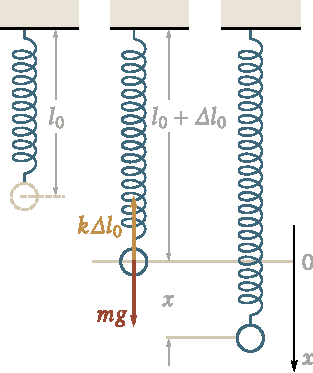
\includegraphics[scale=0.95]{figures/ch_07/fig_7_1.pdf}
		\caption[]{}
		\label{fig:7_1}
	\end{center}
\end{figure}

Để làm ví dụ ta xét hệ gồm một quả cầu khối lượng $m$ được treo vào một lò xo có khối lượng có thể bỏ qua so với $m$ [hình \fig{7_1}].Tại vị tí cân bằng lực $mg$ cân bằng với lực đàn hồi $k\Delta l_0$:
\begin{equation}\label{eq:7_3}
	mg = k\Delta l_0
\end{equation}

\noindent
($\Delta l_0$ là độ dãn của lò xo). Ta sẽ đặc trưng độ dời của quả cầu khỏi vị trí cân bằng bởi tọa độ $x$, thêm vào đó hướng trục $x$ theo đường thẳng đứng xuống dưới, còn điểm không của trục trùng với vị trí cân bằng của quả cầu. Nếu dời quả cầu tới vị trí đặc trưng bằng tọa độ $x$, thì độ dãn của lò xo bằng $\Delta l_0+x$, và hình chiếu của tổng hợp lực lên trục $x$ có giá trị $F=mg-k(\Delta l_0+x)$. Nếu chú ý đến~\eqref{eq:7_3} ta được:
\begin{equation}\label{eq:7_4}
	F = -kx.
\end{equation}

\noindent
Vậy, trong ví dụ đang xét tổng hợp lực của lực hấp dẫn và lực đàn hồi có đặc tính của lực giả đàn hồi.

Ta truyền cho quả cầu một độ dời $x=a$, sau đó ta cho hệ tự thể hiện. Dưới tác dụng của lực giả đàn hồi quả cầu sẽ chuyển động tới vị trí cân bằng với vận tốc tăng nhanh $v=\dot{x}$. Khi đó thé năng của hệ sẽ giảm [hình \fig{7_2}], nhưng lại xuất hiện động năng tăng nhanh\footnote{Khi nghiên cứu về các dao động người ta thường ký hiệu chu kỳ dao động bằng chữ T. Do đó ta ký hiệu động năng bằng chữ $E_k$.} $E_{\text{k}}=m\dot{x}^2/2$ will (bỏ qua khối lượng của lò xo).

\begin{figure}[!htb]
	\begin{center}
		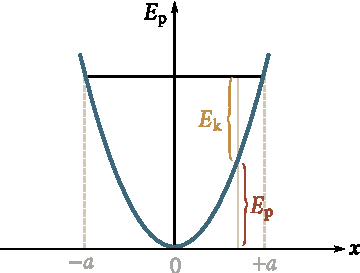
\includegraphics[scale=0.95]{figures/ch_07/fig_7_2.pdf}
		\caption[]{}
		\label{fig:7_2}
	\end{center}
\end{figure}

 Khi tới vị trí cân bằng quả cầu tiếp tục chuyển động theo quán tính. Chuyển động này sẽ bị làm chậm và ngừng lại khi động năng chuyển hoàn toàn thành thế năng, nghĩa là khi độ dời của quả cầu bằng $-a$. Sau đó một quá trình như vậy sẽ xảy ra với chuyển động của quả cầu theo chiều ngược lại. Nếu trong hệ không có ma sát thì năng lượng của hệ phải bảo toàn và quả cầu sẽ chuyển động vĩnh cửu trong các phạm vi từ $x=a$ đến $x=-a$.

Phương trình của định luật Newton thứ hai đối với quả cầu có dạng
\begin{equation}\label{eq:7_5}
	m\ddot{x} = -kx.
\end{equation}

\noindent
Đưa vào ký hiệu
\begin{equation}\label{eq:7_6}
	\omega_0^2 = \frac{k}{m}
\end{equation}

\noindent
Ta biến đổi phương trình \eqn{7_5} như sau:
\begin{equation}\label{eq:7_7}
	\ddot{x} + \omega_0^2 x = 0.
\end{equation}

\noindent
Vì $k/m>0$ nên $\omega_0$ là đại lượng thực.

Vậy khi không có các lực má sát thì chuyển động dưới tác dụng của lực giả đàn hồi được miêu tả bằng phương trình vi phân~\eqref{eq:7_7}.

Trong mọi hệ dao động thực đều có các lực cản mà tác dụng của chúng dẫn tới việc làm giảm năng lượng của hệ. Nếu sự giảm năng lượng không được bù đắp do công của các ngoại lực thì dao động sẽ tắt dần. Trong trường hợp đơn giản nhất và đồng thời hay gặp nhất là lực cản $F^*$ tỷ lệ với độ lớn của vận tốc:
\begin{equation}\label{eq:7_8}
	F_x^* = -r\dot{x}.
\end{equation}

\noindent
Ở đây $r$ là một hằng số được gọi là \textbf{hệ số cản}. Dấu trừ được quy định là lực $\vec{F}^*$ và vận tốc $\vec{v}$ có các chiều ngược nhau; do đó các hình chiếu của chúng trên trục x có các dấu khác nhau.

Phương trình của định luật Newton thứ hai khi có các lực cản có dạng
\begin{equation}\label{eq:7_9}
	m\ddot{x} = -kx - r\dot{x}.
\end{equation}

\noindent
Dùng các ký hiệu
\begin{equation}\label{eq:7_10}
	2\beta = \frac{r}{m}
\end{equation}

\noindent
[so sánh với \eqn{7_6}], ta viết lại phương trình \eqn{7_9} như sau:
\begin{equation}\label{eq:7_11}
	\ddot{x} + 2\beta\dot{x} + \omega_0^2 x = 0.
\end{equation}

\noindent
Phương trình vi phân này miêu tả dao động tắt dần của hệ.

Các dao động miêu tả bằng các phương trình~\eqref{eq:7_7} và~\eqref{eq:7_11} là các dao động tự do (hay các dao động riêng): khi bị đẩy khỏi vị trí cân bằng hoặc khi nhận được một va đập hệ sẽ thực hiện một dao động nếu nó được tự do. Bây giờ giả thử hệ dao động chịu tác dụng ngoại lực biến đổi với thời gian theo định luật điều hòa:
\begin{equation}\label{eq:7_12}
	F_x = F_0 \cos\omega t.
\end{equation}

\noindent
Trong trường hợp này phương trình của định luật Newton thứ hai có dạng
\begin{equation*}
	m\ddot{x} = -kx - r\dot{x} + F_0 \cos\omega t.
\end{equation*}

\noindent
Đưa vào ký hiệu~\eqref{eq:7_6} và~\eqref{eq:7_10} ta viết phương trình này như sau:
\begin{equation}\label{eq:7_13}
	\ddot{x} + 2\beta\dot{x} +\omega_0^2 x = f_0 \cos\omega t
\end{equation}

\noindent
trong đó
\begin{equation}\label{eq:7_14}
	f_0 = \frac{F_0}{m}.
\end{equation}

\noindent
Phương trình~\eqref{eq:7_13} miêu tả dao động cưỡng bức.

Ta biết rằng khi nghiên cứu các dao động có dạng khác nhau ta sẽ đụng chạm với sự cần thiết phải giải các phương trình vi phân dạng
\begin{equation}\label{eq:7_15}
	\ddot{x} + a\dot{x} +bx = f(t)
\end{equation}

\noindent
trong đó $a$ và $b$ là các hằng số, $f(t)$ là một hàm nào đó của $t$. Phương trình có dạng~\eqref{eq:7_15} được gọi là \textbf{phương trình vi phân tuyến tính với các hệ số hằng số}. Trong trường hợp phương trình \eqn{7_7} $a=0$, $b=\omega_0^2$, trong trường hợp phương trình \eqn{7_11} $a=2\beta$, $b=\omega_0^2$. Trong cả hai trường hợp hàm $f(t)$ đồng nhất bằng không: $f(t)\equiv 0$. Trong trường hợp dao động cưỡng bức $f(t)=f_0\cos\omega t$.

Việc giải phương trình \eqn{7_15} được dễ dàng hơn nhiều nếu chuyển qua các đại lượng phức. Do đó trước khi chuyển qua nghiên cứu chi tiết các dao động có dạng khác nhau, ta làm quen một chút với các số phức và các phương pháp giải các phương trình vi phân tuyến tính có các hệ số hằng số.

\section{Số phức}\label{sec:7_3}

Số phức $z$ là số có dạng
\begin{equation}\label{eq:7_16}
	z = x + iy
\end{equation}

\noindent
trong đó $x$ và $y$ là các số thực, $i$ là đơn vị ảo ($i^2=-1$). Số $x$ được gọi là \textbf{phần thực} của số phức $z$. Điều này được viết một cách quy ước dưới dạng $x=\Re\{z\}$. Số $y$ được gọi là \textbf{phần ảo} của $z$ (được viết: $y=\Im\{z\}$). Số
\begin{equation}\label{eq:7_17}
	z^* = x - iy
\end{equation}

\noindent
được gọi là \textbf{số liên hiệp phức} của $x+iy$.

Có thể đối chiếu một điểm trên trục $x$ với số thực $x$. Có thể đối chiếu một điểm trên mặt phẳng có các tọa độ $x$, $y$[hình \fig{7_3}] với số phức $z$. Mỗi điểm trên mặt phẳng xác định một số phức $z$ nào đó. Do đó có thể cho một số phức dưới dạng \eqn{7_16} nhờ các tọa độ Descartes $x$ và $y$ của một điểm tương ứng. Tuy nhiên có thể cho cũng số đó bằng các tọa độ cực $\rho$ và $\varphi$. Giữa cả hai cặp tọa độ có các hệ thức:
\begin{equation}\label{eq:7_18}
	\begin{cases}
		x = \rho\cos\varphi,\quad\quad\quad y = \rho\sin\varphi,\\
		\rho = \left(x^2+y^2\right)^{1/2},\quad \varphi = \arctan\dfrac{y}{x}.
	\end{cases}
\end{equation}

Khoảng cách từ gốc tọa độ đến điểm mô tả số $z$ được gọi là \textbf{module} của số phức (được ký hiệu là $|z|$). Rõ ràng là
\begin{equation}\label{eq:7_19}
	|z| = \rho = \sqrt{x^2+y^2}.
\end{equation}

\noindent
Số $\varphi$ được gọi là \textbf{argument} của số phức $z$.

Nếu chú ý tới hệ thức~\eqref{eq:7_18} thì có thể biểu diễn số phức dưới dạng lượng giác:
\begin{equation}\label{eq:7_20}
	z = \rho(\cos\varphi + i\sin\varphi).
\end{equation}

Hai số phức $z_1=x_1+iy_1$ và $z_2=x_2+iy_2$ được coi là bằng nhau nếu các phần thực và ảo của chúng tương ứng bằng nhau:
\begin{equation}\label{eq:7_21}
	z_1 = z_2\,\, \text{nếu}\,\, x_1 = x_2\,\, \text{và}\,\, y_1 = y_2.
\end{equation}

\noindent
Các module của hai số phức bằng nhau là bằng nhau, còn các argument có thể chỉ khác nhau bởi một số hạng, bội của $2\pi$:
\begin{equation}\label{eq:7_22}
	\rho_1 = \rho_2,\quad \varphi_1 = \varphi_2\pm 2k\pi
\end{equation}

\noindent
trong đó $k$ là số nguyên.

\begin{figure}[!htb]
	\begin{center}
		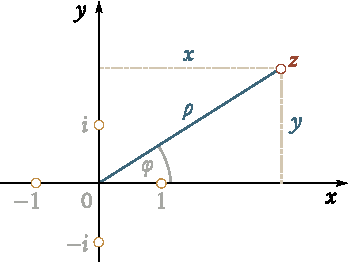
\includegraphics[scale=0.95]{figures/ch_07/fig_7_3.pdf}
		\caption[]{}
		\label{fig:7_3}
	\end{center}
\end{figure}

Từ các biểu thức~\eqref{eq:7_16} và~\eqref{eq:7_17} rõ ràng trong trường hợp khi $z^*=z$, thì phần ảo của $z$ là số không, nghĩa là số $z$ là thuần túy thực. Vậy có thể viết điều kiện $z$ là số thực dưới dạng
\begin{equation}\label{eq:7_23}
	z^* = z.
\end{equation}

Trong toán học người ta đã chứng minh hệ thức
\begin{equation}\label{eq:7_24}
	e^{i\varphi} = \cos\varphi + i\sin\varphi
\end{equation}

\noindent
nó được gọi là \textbf{công thức Euler}. Nếu thay $\varphi$ trong công thức này bằng $-\varphi$ và chú ý rằng $\cos(-\varphi)=\cos\varphi$, còn $\sin(-\varphi)=-sin\varphi$ ta có hệ thức
\begin{equation}\label{eq:7_25}
	e^{-i\varphi} = \cos\varphi - i\sin\varphi.
\end{equation}

Cộng các biểu thức~\eqref{eq:7_24} và~\eqref{eq:7_25} và giải hệ thức tìm được đối với $\cos\varphi$. Kết quả ra có
\begin{equation}\label{eq:7_26}
	\cos\varphi = \frac{1}{2}\left(e^{i\varphi} + e^{-i\varphi}\right).
\end{equation}

\noindent
Trừ \eqn{7_25} với~\eqref{eq:7_24} ta được $\sin\varphi=\left(e^{i\varphi} + e^{-i\varphi}\right)/2i$.

Nhờ công thức~\eqref{eq:7_24} có thể viết số phức dưới dạng mũ:
\begin{equation}\label{eq:7_27}
	z = \rho e^{i\varphi}
\end{equation}

\noindent
[xem \eqn{7_20}]. Số liên hiệp phức ở dạng mũ có dạng
\begin{equation}\label{eq:7_28}
	z^* = \rho e^{-i\varphi}.
\end{equation}

\noindent
Khi cộng các số phức, người ta cộng riêng các phần thực và ảo của chúng:
\begin{equation}\label{eq:7_29}
	z_1 + z_2 = (x_1 + x_2) + i(y_1 + y_2).
\end{equation}

Thực hiện phép nhân các số phức được thuận lợi nếu lấy các số này ở dạng mũ:
\begin{equation}\label{eq:7_30}
	z = z_1 z_2 = \rho_1 e^{i\varphi_1} \rho_2 e^{i\varphi_2} = \rho_1\rho_2 e^{i(\varphi_1 + \varphi_2}.
\end{equation}

\noindent
Các module của các số phức được nhân với nhau, còn các argument được cộng lại:
\begin{equation}\label{eq:7_31}
	\rho = \rho_1\rho_2,\quad \varphi = \varphi_1 + \varphi_2.
\end{equation}

\noindent
Phép chia các số phức cũng được thực hiện một cách tương tự:
\begin{equation}\label{eq:7_32}
	z = \frac{z_1}{z_2} = \frac{\rho_1 e^{i\varphi_1}}{\rho_2 e^{i\varphi_2}} = \frac{\rho_1}{\rho_2}e^{i(\varphi_1 - \varphi_2}.
\end{equation}

Nếu chú ý tới các công thức~\eqref{eq:7_27} và~\eqref{eq:7_28} thì dễ dàng thu được
\begin{equation}\label{eq:7_33}
	zz^* = \rho^2
\end{equation}

\noindent
(bình phương module của một số phức thì bằng tích của số này với số liên hiệp phức của nó).

\section{Các phương trình vi phân tuyến tính}\label{sec:7_4}

Phương trình có dạng
\begin{equation}\label{eq:7_34}
	\ddot{x} + a\dot{x} + bx = f(t)
\end{equation}

\noindent
trong đó $a$ và $b$ là các hằng số, $f(t)$ là hàm đã cho của $t$, được gọi là \textbf{phương trình vi phân tuyến tính cấp hai với các hệ số hằng số}. Các hằng số $a$ và $b$ có thể đều bằng không.

Nếu hàm $f(t)$ là đồng nhất bằng không ($f(t)\equiv 0$) thì phương trình được gọi là phương trình \textbf{thuần nhất}, trong trương hợp ngược lại --- phương trình \textbf{không thuần nhất}. Phương trình thuần nhất có dạng
\begin{equation}\label{eq:7_35}
	\ddot{x} + a\dot{x} + bx = 0.
\end{equation}

Nghiệm của mọi phương trình vi phân cấp hai (nghĩa là với đạo hàm có cấp cao nhất là 2) chứa hai hằng số tùy ý $C_1$ và $C_2$. Điều này có thể hiểu được, nếu để ý rằng xác định hàm theo đạo hàm cấp hai của nó được thực hiện bằng cách lấy tích phân hai lần. Với mỗi lần lấy tích phân sẽ xuất hiện một hằng số tích phân. Để làm ví dụ ta xét phương trình
\begin{equation}\label{eq:7_36}
	\ddot{x} = 0.
\end{equation}

\noindent
Lấy tích phân phương trình này cho $\dot{x}=C_1$. Lấy tích phân lần thứ hai dẫn tới hàm
\begin{equation}\label{eq:7_37}
	x = C_1 t + C_2.
\end{equation}

\noindent
Dễ dàng khẳng định rằng với các giá trị bất kỳ của các hằng số $C_1$ và $C_2$ hàm~\eqref{eq:7_37} thỏa mãn phương trình \eqn{7_36}.

Nếu cho các hằng số $C_1$ và $C_2$ các giá trị xác định ta được nghiệm gọi là \textbf{nghiệm riêng} của phương trình vi phân. Chẳng hạn, hàm $5t+3$ là một trong các nghiệm riêng của phương trình \eqn{7_36}.

Tập hợp tất cả các nghiệm không ngoại trừ các nghiệm riêng được gọi là \textbf{nghiệm tổng quát} của phương trình vi phân. Nghiệm tổng quát của phương trình \eqn{7_36} có dạng \eqn{7_37}.

Trong lý thuyết các phương trình vi phân tuyến tính người ta chứng minh rằng nếu $x_1$ và $x_2$ là các nghiệm độc lập tuyến tính\footnote{Các hàm $x_1$ và $x_2$ được gọi là các hàm độc lập tuyến tính với nhau nếu hệ thức $\alpha_1 x_1+\alpha_2 x_2=0$ chỉ được nghiệm đúng trong trường hợp mà $\alpha_1$ và $\alpha_2$ đều bằng không.} của phương trình thuần nhất~\eqref{eq:7_35} thì có thể biểu diễn nghiệm tổng quát của phương trình này dưới dạng
\begin{equation}\label{eq:7_38}
	x = C_1 x_1 + C_2 x_2
\end{equation}

\noindent
trong đó $C_1$ và $C_2$ là các hằng số tùy ý.

Giả thử $x_{\text{n}}(t, C_1, C_2)$ là nghiệm tổng quát của phương trình không thuần nhất~\eqref{eq:7_34} (các hằng số tùy ý $C_1$ và $C_2$ tham gia vào nghiệm này với tư cách là các tham số), còn $x_{\text{n}}(t)$ là một trong những nghiệm riêng của phương trình đó (nó không chứa các hằng số tùy ý). Ta đưa vào ký hiệu
\begin{equation*}
	x(t, C_1, C_2) = x_{\text{n}}(t, C_1, C_2) - x_{\text{n}}(t).
\end{equation*}

\noindent
Khi đó có thể biểu diễn nghiệm tổng quát của phương trình không thuần nhất dưới dạng
\begin{equation}\label{eq:7_39}
	x_{\text{n}}(t, C_1, C_2) = x_{\text{n}}(t) + x(t, C_1, C_2).
\end{equation}

\noindent
Với các giá trị bất kỳ của các hằng số $C_1$ và $C_2$ hàm~\eqref{eq:7_39} thỏa mãn phương trình \eqn{7_34}. Do đó có thể viết hệ thức:
\begin{equation*}
	\ddot{x}_{\text{n}}(t) + \ddot{x}(t, C_1, C_2) + a\dot{x}_{\text{n}}(t) + a\dot{x}(t, C_1, C_2) + bx_{\text{n}}(t) + bx(t, C_1, C_2) = f(t).
\end{equation*}

\noindent
Nếu nhóm các số hạng lại ta có:
\begin{equation}\label{eq:7_40}
	\ddot{x}(t, C_1, C_2) + a\dot{x}(t, C_1, C_2) + bx(t, C_1, C_2) + [\ddot{x}_{\text{n}}(t) + a\dot{x}_{\text{n}}(t) + bx_{\text{n}}(t)] = f(t).
\end{equation}

Nghiệm riêng $x_{\text{n}}(t)$ cũng thỏa mãn phương trình \eqn{7_34}. Do đó biểu thức nằm trong các dấu móc vuông ở vế trái của hệ thức \eqn{7_40} bằng vế phải của hệ thức đó. Từ đó suy ra rằng hàm $x(t, C_1, C_2)$ phải thỏa mãn điều kiện
\begin{equation*}
	\ddot{x}(t, C_1, C_2) + a\dot{x}(t, C_1, C_2) + bx(t, C_1, C_2) = 0
\end{equation*}

\noindent
tức là nó là nghiệm tổng quát của phương trình thuần nhất~\eqref{eq:7_35}. Như vậy, ta đã đi tới một định lý rất bổ ích: \textit{nghiệm tổng quát của phương trình không thuần nhất bằng tổng của nghiệm tổng quát của phương trình thuần nhất tương ứng và một nghiệm riêng nào đó của phương trình không thuần nhất}:
\begin{equation}\label{eq:7_41}
	x_{\text{tq,ktn}} = x_{\text{tq,tn}} + x_{\text{r,ktn}}.
\end{equation}

\noindent
Người ta giải các phương trình vi phân tuyến tính thuần nhất nhờ phép thế
\begin{equation}\label{eq:7_42}
	x(t) = e^{\lambda t}
\end{equation}

\noindent
trong đó $\lambda$ là một đại lượng không đổi. Lấy vi phân hàm~\eqref{eq:7_42} cho
\begin{equation}\label{eq:7_43}
	\dot{x}(t) = \lambda e^{\lambda t},\quad \ddot{x}(t) = \lambda^2 e^{\lambda t}.
\end{equation}

\noindent
Thế các biểu thức~\eqref{eq:7_42} và~\eqref{eq:7_43} vào phương trình~\eqref{eq:7_35}, sau khi giản ước nhân tử khác không $e^{\lambda t}$, dẫn tới phương trình đại số
\begin{equation}\label{eq:7_44}
	\lambda^2 + a\lambda + b = 0.
\end{equation}

\noindent
phương trình này được gọi là \textbf{phương trình đặc trưng}. Các nghiệm của phương trình này là các giá trị của $\lambda$ mà hàm~\eqref{eq:7_42} thỏa mãn phương trình~\eqref{eq:7_35}.

Nếu các nghiệm của phương trình \eqn{7_44} không trùng nhau ($\lambda_1\neq\lambda_2$) thì các hàm $e^{\lambda_1 t}$ và $e^{\lambda_2 t}$ sẽ độc lập tuyến tính với nhau. Do đó, theo \eqn{7_38} có thể viết nghiệm tổng quát của phương trình\eqn{7_35} dưới dạng
\begin{equation}\label{eq:7_45}
	x = C_1 e^{\lambda_1 t} + C_2 e^{\lambda_2 t}.
\end{equation}

\noindent
Có thể chứng tỏ rằng trong trường hợp khi $\lambda_1=\lambda_2=\lambda$ nghiệm tổng quát của phương trình \eqn{7_35} có dạng như sau:
\begin{equation}\label{eq:7_46}
	x = C_1 e^{\lambda t} + C_2 t e^{\lambda t}.
\end{equation}

Ta giả thử rằng các hệ số $a$ và $b$ là thực, còn hàm trong vế phải của phương trình \eqn{7_34} là phức. Nếu biểu diễn hàm này dưới dạng $f(t)+i\varphi(t)$, ta đi tới phương trìnhtrình:
\begin{equation}\label{eq:7_47}
	\ddot{z} + a\dot{z} + bz = f + i\varphi
\end{equation}

\noindent
(ta đã ký hiệu hàm phải tìm bằng chữ $z$). Nghiệm của phương trình rõ ràng sẽ là phức. Sau khi viết nghiệm dưới dạng $z(t)=x(t)+iy(t)$, ta thế nó vào phương trình \eqn{7_47}. Kết quả ta có:
\begin{equation}\label{eq:7_48}
	\ddot{x} + i\ddot{y} + a\dot{x} + ai\dot{y} + bx + biy = f + i\varphi.
\end{equation}

\noindent
Ở các số phức bằng nhau thì các phần thực và các phần ảo tương ứng bằng nhau [xem \eqn{7_21}]. Do đó, phương trình \eqn{7_48} được phân thành hai phương trình độc lập:
\begin{equation}\label{eq:7_49}
	\ddot{x} + a\dot{x} + bx = f(t),\quad \ddot{y} + a\dot{y} + by = \varphi
\end{equation}

\noindent
trong đó phương trình đầu trùng với phương trình \eqn{7_34}. Tính chất này của phương trình \eqn{7_48} cho phép sử dụng thủ thuật sau đây, đôi khi làm giảm nhẹ đáng kể các tính toán. Giả thử phương trình \eqn{7_34} do ta giải có vế phải là thực. Nếu thêm vào nó một hàm ảo tùy ý, ta đưa phương trình về dạng \eqn{7_47}. Sau đó bằng cách tìm nghiệm phức của phương trình, ta lấy phần thực của nó. Nó sẽ là nghiệm của phương trình xuất phát [\eqn{7_34}].

\section{Dao động điều hòa}\label{sec:7_5}

Hãy xét một dao động được mô tả bằng phương trình
\begin{equation*}
	\ddot{x} + \omega_0^2 x = 0\tag{\ref{eq:7_7} xem lại}.
\end{equation*}

\noindent
Dao động đó được thực hiện bởi vật có khối lượng $m$ chỉ chịu tác dụng của một lực giả đàn hồi $F=-kx$. Hệ số của $x$ trong phương trình \eqn{7_7} có giá trị
\begin{equation*}
	\omega_0^2 = \frac{k}{m}.\tag{\ref{eq:7_6} xem lại}.
\end{equation*}

Thế biểu thức $x=e^{\lambda t}$ [xem \eqn{7_42}] vào \eqn{7_7}, ta đi tới phương trình đặc trưng
\begin{equation}\label{eq:7_50}
	\lambda^2 + \omega_0^2 = 0.
\end{equation}

\noindent
Phương trình này có các nghiệm ảo: $\lambda_1=+i\omega_0$ và $\lambda_2=-i\omega_0$. Theo \eqn{7_45} nghiệm tổng quát của phương trình \eqn{7_7} có dạng
\begin{equation}\label{eq:7_51}
	x = C_1 e^{i\omega_0 t} + C_2 e^{-i\omega_0 t}
\end{equation}

\noindent
trong đó $C_l$ và $C_2$ là các hằng số phức.

Hàm $x(t)$ mô tả dao động phải là hàm thực. Muốn vậy cần phải chọn các hệ số $C_l$ và $C_2$ trong \eqn{7_51} so cho thực hiện được điều kiện [xem \eqn{7_23}]:
\begin{equation}\label{eq:7_52}
	C_1^* e^{-i\omega_0 t} + C_2^* e^{i\omega_0 t} = C_1 e^{i\omega_0 t} + C_2 e^{-i\omega_0 t}
\end{equation}

\noindent
[ta đã cân bằng biểu thức~\eqref{eq:7_51} với liên hợp phức của nó]. Hệ thức~\eqref{eq:7_52} sẽ được thực hiện nếu $C_1=C_2^*$ (trong trường hợp này $C_2=C_1^*$). Ta biểu diễn các hệ số $C_l$ và $C_2$ thỏa mãn điều kiện đó dưới dạng mũ [xem \eqn{7_17}], bằng cách ký hiệu module của chúng là $A/2$, còn argument bằng chữ $\alpha$:
\begin{equation}\label{eq:7_53}
	C_1 = \frac{A}{2}e^{i\alpha},\quad 	C_2 = \frac{A}{2}e^{-i\alpha}.
\end{equation}

\noindent
Thế các biểu thức này vào \eqn{7_51} ta được
\begin{equation}\label{eq:7_54}
	x = \frac{A}{2}\left[e^{i(\omega_0 t+\alpha)} + e^{-i(\omega_0 t+\alpha)}\right] = A\cos(\omega_0 t + \alpha)
\end{equation}

\noindent
[xem \eqn{7_26}]. Vậy nghiệm tổng quát của phương trình \eqn{7_49} có dạng
\begin{equation}\label{eq:7_55}
	x = A\cos(\omega_0 t + \alpha)
\end{equation}

\noindent
trong đó $A$ và $\alpha$ là các hằng số tùy ý \footnote{Còn có thể viết nghiệm của phương trình \eqn{7_7} bằng hai cách. Biến đổi biểu thức \eqn{7_55} theo công thức đối với cosin của tổng: $x = A(\cos\alpha\cos\omega_0 t - \sin\alpha\sin\omega_0 t)$ và đưa vào ký hiệu $c_1=A\cos\alpha$ và $c_2=-A\sin\alpha$. Khi đó có thể biểu diễn hàm $x(t)$ dưới dạng $x=c_1\cos\omega_0 t+c_2\sin\omega_0 t$, trong đó $c_1$ và $c_2$ là những hằng số tùy ý. Cuối cùng, nếu dùng công thức \eqn{7_24} có thể viết biểu thức \eqn{7_55} như sau: $x=\Re\left\{Ae^{i(\omega_0 t+\alpha)}\right\}$.}.

Vậy độ dời $x$ biến đổi theo thời gian theo quy luật cosine. Do đó, chuyển động của một hệ chịu tác dụng của lực có dạng $F=-kx$ là một dao động điều hòa.

\begin{figure}[!htb]
	\begin{center}
		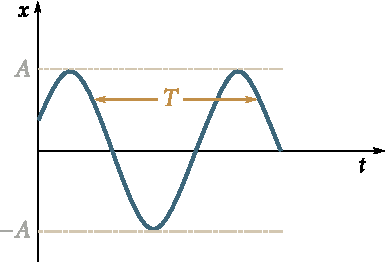
\includegraphics[scale=0.95]{figures/ch_07/fig_7_4.pdf}
		\caption[]{}
		\label{fig:7_4}
	\end{center}
\end{figure}

Đồ thị của dao động điều hòa, nghĩa là đồ thị của hàm~\eqref{eq:7_55}, được trình bày trên hình \fig{7_4}. Trên trục nằm ngang người ta đặt thời gian $t$, trên trục thẳng đứng là độ dời $x$. Vì cosine biến đổi trong phạm vi từ $-1$ đến $1$ nên các giá trị của $x$ nằm trong phạm vi từ $-A$ đến $A$.

Độ lớn của độ lệch lớn nhất của hệ khỏi vị trí cân bằng được gọi là \textbf{biên độ} dao động. Biên độ $A$ là một đại lượng dương không đổi. Giá trị của nó được xác định bằng độ lớn của độ lệch ban đầu hoặc của sự va đập làm hệ rời khỏi vị trí cân bằng.

Đại lượng ($\omega_0 t+\alpha$) đứng dưới dấu cosine được gọi là \textbf{pha} của dao động. Hằng số $\alpha$ là giá trị của pha tại thời điểm $t=0$ và được gọi là \textbf{pha ban đầu} của dao động. Khi thay đổi gốc tính thời gian thì cả $\alpha$ cũng sẽ thay đổi. Do đó giá trị của pha ban đầu được xác định bằng sự chọn gốc tính thời gian. Vì giá trị của $x$ không thay đổi khi thêm vào hoặc bớt đi từ pha một số nguyên lần $2\pi$ nên bao giờ cũng có thể tìm cách để cho pha ban đầu có module nhỏ hơn $\pi$. Do đó thường người ta chỉ xét các giá trị của $\alpha$ nằm trong các phạm vi từ $-\pi$ đến $+\pi$.

Vì cosine là hàm tuần hoàn với chu kỳ $2\pi$ nên các trạng thái khác nhau\footnote{Hãy nhớ rằng trạng thái của một hệ cơ học được đặc trưng bởi các giá trị của các tọa độ và vận tốc của các vật tạo thành hệ.}của hệ thực hiện dao động điều hòa được lặp lại sau một khoảng thời gian $T$ mà trong đó pha của dao động nhận số gia bằng $2\pi$ (\fig{7_4}). Khoảng thời gian $T$ này được gọi là \textbf{chu kỳ} dao động. Nó có thể xác định từ điều kiện sau: $|\omega_0(t+T)+\alpha|=|\omega_0 t+\alpha|+2\pi$, từ đó
\begin{equation}\label{eq:7_56}
	T = \frac{2\pi}{\omega_0}.
\end{equation}

Số dao động trong một đơn vị thời gian được gọi là \textbf{tần số} dao động $\nu$. Rõ ràng là tần số $\nu$ liên hệ với khoảng thời gian $T$ của dao động bằng hệ thức sau đây:
\begin{equation}\label{eq:7_57}
	\nu = \frac{1}{T}.
\end{equation}

\noindent
Tần số của một dao động có chu kỳ bằng \SI{1}{\second} được lấy làm đơn vị của tần số. Đơn vị này được gọi là hertz (\si{\hertz}). Tần số  \SI{e3}{\hertz} được gọi là một kilohertz (\si{\kilo\hertz}), \SI{e6}{\hertz} là một megahertz (\si{\mega\hertz}).

Từ \eqn{7_56} suy ra rằng
\begin{equation}\label{eq:7_58}
	\omega_0 = \frac{2\pi}{T}.
\end{equation}

\noindent
Vậy $\omega_0$ cho số dao động trong $2\pi$ giây. Người ta gọi đại lượng $\omega_0$ là \textbf{tần số tròn} hoặc \textbf{tần số cyclic}. Nó liên hệ với tần số thông thường $\nu$ bằng hệ thức
\begin{equation}\label{eq:7_59}
	\omega_0 = 2\pi\nu.
\end{equation}

Nếu lấy vi phân \eqn{7_55} theo thời gian, ta được biểu thức đối với vận tốc
\begin{equation}\label{eq:7_60}
	v = \dot{x} = -A\omega_0\sin(\omega_0 t + \alpha) = A\omega_0\cos\left(\omega_0 t + \alpha + \frac{\pi}{2}\right).
\end{equation}

\noindent
Như đã thấy trong \eqn{7_60} vận tốc cũng biến thiên theo quy luật điều hòa, thêm vào đó biên độ của vận tốc bằng $A\omega_0$. Từ sự so sánh~\eqref{eq:7_55} và~\eqref{eq:7_60} suy ra rằng vận tốc nhanh pha hơn độ dời là $\pi/2$.

Nếu lấy vi phân \eqn{7_60} một lần nữa theo thời gian, ta tìm được biểu thức cho gia tốc:
\begin{equation}\label{eq:7_61}
	a = \ddot{x} = -A\omega_0^2\cos(\omega_0 t + \alpha) = A\omega_0^2\cos(\omega_0 t + \alpha + \pi).
\end{equation}

\noindent
Như suy ra từ \eqn{7_61}, gia tốc và độ dời là ngược pha nhau. Điều này có nghĩa là tại thời điểm khi độ dời đạt tới giá trị dương lớn nhất thì gia tốc đạt tới giá trị âm lớn nhất về độ lớn và ngược lại.

Trên hình~\ref{fig:7_5} người ta dựng các đồ thị của độ dời, vận tốc và gia tốc.

\begin{figure}[!htb]
	\begin{center}
		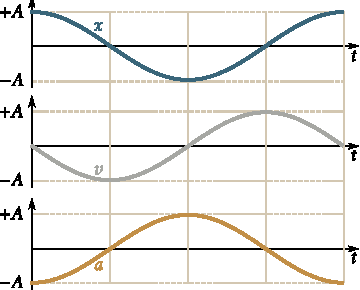
\includegraphics[scale=0.95]{figures/ch_07/fig_7_5.pdf}
		\caption[]{}
		\label{fig:7_5}
	\end{center}
\end{figure}

Mỗi dao động cụ thể được đặc trưng bởi các giá trị xác định của biên độ $A$ và của pha ban đầu $\alpha$. Các giá trị của các đại lượng này đối với dao động đã cho có thể được xác định từ các điều kiện ban đầu, nghĩa là theo các giá trị của độ lệch $x_0$ và của vận tốc $v_0$ tại thời điểm ban đầu. Thực vậy, trong~\eqref{eq:7_55} và~\eqref{eq:7_60} nếu đặt $t=0$ ta thu được hai phương trình::
\begin{equation*}
	x_0 = A\cos\alpha,\quad v_0 = -A\omega_0\sin\alpha
\end{equation*}

\noindent
từ các phương trình này ta tìm được
\begin{align}
	A &= \left(x_0^2 + \frac{v_0^2}{\omega_0^2}\right)^{1/2}, \label{eq:7_62}\\
	\tan\alpha &= -\frac{v_0}{x_0\omega_0}.\label{eq:7_63}
\end{align}

\noindent
Phương trình~\eqref{eq:7_63} được thỏa mãn bởi hai giá trị $\alpha$ nằm trong khoảng từ $-\pi$ đến $+\pi$. Trong các giá trị này phải lấy giá trị nào mà ta có được các dấu đúng ở cosine và sine.

Lực giả đàn hồi là lực bảo toàn. Do đó năng lượng toàn phần của dao động điều hòa vẫn phải không đổi. Trong quá trình dao động xảy ra sự chuyển động xảy ra sự chuyển hóa động năng thành thế năng và ngược lại, thêm vào đó tại những thời điểm độ lệch khỏi vị trí cân bằng là lớn nhất thì năng lượng toàn phần $E$ chỉ gồm có thế năng, đạt tới giá trị lớn nhất $E_{\text{p,max}}$ của nó:
\begin{equation}\label{eq:7_64}
	E = E_{\text{p,max}} = \frac{kA^2}{2}.
\end{equation}

\noindent
Khi hệ đi qua vị trí cân bằng năng lượng toàn phần của hệ chỉ gồm có động năng đạt tới giá trị lớn nhất $E_{\text{k,max}}$ của nó vào những thời điểm đó:
\vspace{-12pt}
\begin{equation}\label{eq:7_65}
	E = E_{\text{k,max}} = \frac{mv_{\text{max}}^2}{2} = \frac{mA^2\omega_0^2}{2}
\end{equation}

\noindent
(trên đây đã chứng tỏ rằng biên độ của vận tốc là bằng $A\omega_0$). Các biểu thức~\eqref{eq:7_64} và~\eqref{eq:7_65} đều bằng nhau, vì theo \eqn{7_6} $m\omega_0^2=k$.

Ta hãy tìm hiểu xem động năng và thế năng của một dao động điều hòa biến đổi theo thời gian như thế nào. Động năng là bằng [xem \eqn{7_60} đối với $\dot{x}$]
\begin{equation}\label{eq:7_66}
	E_{\text{k}} = \frac{m\dot{x}^2}{2} = \frac{mA^2\omega_0^2}{2}\sin^2(\omega_0 t + \alpha).
\end{equation}

\noindent
Thế năng được biểu thị bằng công thức
\begin{equation}\label{eq:7_67}
	E_{\text{p}} = \frac{kx^2}{2} = \frac{kA^2}{2}\cos^2(\omega_0 t + \alpha).
\end{equation}

\noindent
Cộng~\eqref{eq:7_66} với~\eqref{eq:7_67} và chú ý rằng $m\omega_0^2=k$, ta thu được công thức đối với năng lượng toàn phần:
\begin{equation}\label{eq:7_68}
	E = E_{\text{k}} + E_{\text{p}}= \frac{kA^2}{2} = \frac{mA^2\omega_0^2}{2}
\end{equation}

\noindent
[so sánh với~\eqref{eq:7_64} và~\eqref{eq:7_65}]. Vậy năng lượng toàn phần của dao động điều hòa thực sự là không đổi.

\begin{figure}[!htb]
	\begin{center}
		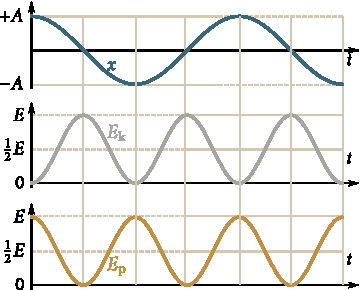
\includegraphics[scale=0.95]{figures/ch_07/fig_7_6.pdf}
		\caption[]{}
		\label{fig:7_6}
	\end{center}
\end{figure}

Dùng các công thức lượng giác đã biết có thể biểu diễn các biểu thức đối với $E_{\text{k}}$ và $E_{\text{p}}$ dưới dạng
\begin{align}
	E_{\text{k}} &= E\sin^2(\omega_0 t + \alpha) = E \left\{\frac{1}{2} - \frac{1}{2}\cos[2(\omega_0 t + \alpha)]\right\}\label{eq:7_69}\\
	E_{\text{p}} &= E\cos^2(\omega_0 t + \alpha) = E \left\{\frac{1}{2} + \frac{1}{2}\cos[2(\omega_0 t + \alpha)]\right\}\label{eq:7_70}
\end{align}

\noindent
trong đó $E$ là năng lượng toàn phần của hệ. Từ các công thức này rõ ràng là $E_{\text{k}}$ và $E_{\text{p}}$ biến đổi với tần số $2\omega_0$, nghĩa là với tần số hai lần cao hơn tần số của dao động điều hòa. Trên hình~\ref{fig:7_6} người ta dựng các đồ thị của $x$, $E_{\text{k}}$ và $E_{\text{p}}$.



Giá trị trung bình của bình phương sine và bình phương cosine, như đã biết, bằng một nửa. Do đó giá trị trung bình của $E_{\text{k}}$ trùng với giá trị trung bình của $E_{\text{p}}$ và bằng $E/2$.

\section{Con lắc}\label{sec:7_6}

Trong vật lý người ta hiểu con lắc là một vật rắn thực hiện dao động xung quanh một điểm hay một trục cố định dưới tác dụng của trọng lực. Người ta thường phân biệt con lắc toán học và con lắc vật lý.

Con lắc toán học là một hệ được lý tưởng hóa gồm một sợi dây không trọng lượng và không dãn treo một khối lượng được tập trung và một điểm. Khá gần với con lắc toán học là một quả cầu nặng không lớn treo vào một sợi dây mảnh dài.

\begin{figure}[!htb]
	\begin{center}
		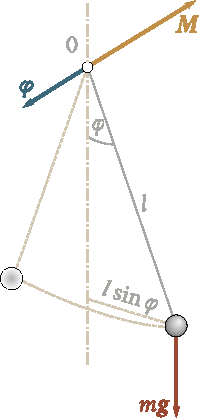
\includegraphics[scale=0.95]{figures/ch_07/fig_7_7.pdf}
		\caption[]{}
		\label{fig:7_7}
	\end{center}
\end{figure}

Độ lệch của con lắc khỏi vị trí cân bằng sẽ đặc trưng bởi góc $\varphi$ được tạo bởi sợi dây với đường thẳng đứng (\fig{7_7}).Khi con lắc lệch khỏi vị trí cân bằng sẽ xuất hiện moment quay $M$, về độ lớn bằng $mgl\sin\varphi$ ($m$ là khối lượng, còn $l$ là độ dài con lắc). Nó có hướng sao cho hướng con lắc trở về vị trí cân bằng, và về mặt này nó tương tự như lực giả đàn hồi. Do đó cũng như độ dời và lực giả đàn hồi, cần viết thêm cho moment quay $M$ và độ dời góc $\varphi$ các dấu ngược lại\footnote{Nếu coi $\varphi$ như một vector liên hệ với chiều quay bằng quy tắc cái đinh ốc thuận (điều này đạt được với các $\varphi$ nhỏ), thì có thể giải thích sự mâu thuẫn của các dấu ở trước $M$ và $\varphi$ là các vector $\vec{M}$ và $\vec{\varphi}$ hướng về các phía ngược nhau (\fig{7_7}).}. Do đó biểu thức cho moment quay có dạng
\begin{equation}\label{eq:7_71}
	M = -mgl\sin\varphi.
\end{equation}

Đối với con lắc ta viết phương trình động lực học của chuyển động quay. Nếu ký hiệu gia tốc góc bằng $\ddot{\varphi}$ và chú ý là moment quán tính của con lắc bằng $ml^2$, ta được:
\begin{equation*}
	ml^2\ddot{\varphi} = -mgl\sin\varphi.
\end{equation*}

\noindent
Có thể đưa phương trình này về dạng:
\begin{equation}\label{eq:7_72}
	\ddot{\varphi} + \frac{g}{l}\sin\varphi = 0.
\end{equation}

Ta chỉ giới hạn ở việc khảo sát các dao động bé. Trong trường hợp này có thể đặt $\sin\varphi\approx\varphi$. Ngoài ra, nếu đưa vào ký hiệu
\begin{equation}\label{eq:7_73}
	\frac{g}{l} = \omega_0^2
\end{equation}

\noindent
ta sẽ đi tới phương trình
\begin{equation}\label{eq:7_74}
	\ddot{\varphi} + \omega_0^2\varphi = 0
\end{equation}

\noindent
nó đồng nhất với phương trình \eqn{7_7}. Nghiệm của nó có dạng
\begin{equation}\label{eq:7_75}
	\varphi = A\cos(\omega_0 t + \alpha).
\end{equation}

\noindent
Do đó với các dao động bé, độ lệch góc của con lắc toán học biến đổi với thời gian theo định luật điều hòa.

Như suy ra từ~\eqref{eq:7_73}, tần số dao động của con lắc toán học chỉ phụ thuộc vào độ dài của con lắc và vào gia tốc trọng trường mà không phụ thuộc vào khối lượng con lắc. Theo công thức~\eqref{eq:7_56}, căn cứ vào~\eqref{eq:7_73} ta thu được biểu thức đã biết từ giáo trình phổ thông đối với chu kỳ dao động của con lắc toán học:
\begin{equation}\label{eq:7_76}
	T = 2\pi\left(\frac{l}{g}\right)^{1/2}.
\end{equation}

Chú ý rằng nếu giải phương trình \eqn{7_72} có thể tìm được cho chu kỳ dao động công thức sau:
\begin{equation}\label{eq:7_77}
	T = 2\pi\left(\frac{l}{g}\right)^{1/2}\left\{1 + \left(\frac{1}{2}\right)^2 \sin^2\frac{A}{2} + \left(\frac{1}{2}\times\frac{3}{4}\right)^2\sin^4\frac{A}{2} + \ldots\right\}.
\end{equation}

\noindent
trong đó $A$ là biên độ dao động, nghĩa là góc lớn nhất mà con lắc lệch khỏi vị trí cân bằng.

\begin{figure}[!htb]
	\begin{center}
		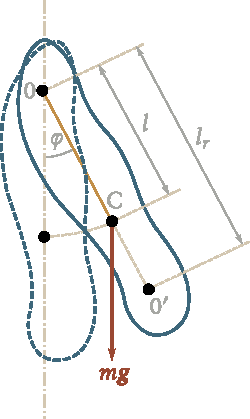
\includegraphics[scale=0.9]{figures/ch_07/fig_7_8.pdf}
		\caption[]{}
		\label{fig:7_8}
	\end{center}
\end{figure}

Nếu không thể biểu diễn vật dao động như một chất điểm thì con lắc được gọi là con lắc vật lý. Khi con lắc lệch khỏi vị trí cân bằng một góc $\varphi$ sẽ xuất hiện một moment quay có xu hướng làm con lắc quay về vị trí cân bằng. Moment này bằng
\begin{equation}\label{eq:7_78}
	M = -mgl\sin\varphi
\end{equation}

\noindent
trong đó $m$ là khối lượng của con lắc, còn $l$ là khoảng cách giữa điểm treo $O$ và khối tâm $C$ của con lắc (\fig{7_8}). Dấu ``$-$'' có cùng ý nghĩa như trong trường hợp của công thức \eqn{7_71}.

Nếu ký hiệu moment quán tính của con lắc đối với trục đi qua điểm treo bằng chữ $I$ thì có thể viết:
\begin{equation}\label{eq:7_79}
	I\ddot{\varphi} = -mgl\sin\varphi.
\end{equation}

\noindent
Trong trường hợp các dao động bé \eqn{7_79} chuyển về phương trình \eqn{7_74} mà ta đã biết:
\begin{equation*}
	\ddot{\varphi} +\omega_0^2\varphi = 0.
\end{equation*}

\noindent
Trong trường hợp này $\omega_0^2$ ký hiệu cho các đại lượng sau:
\begin{equation}\label{eq:7_80}
	\omega_0^2 = \frac{mgl}{I}.
\end{equation}

Từ các phương trình~\eqref{eq:7_74} và~\eqref{eq:7_80} suy ra rằng với các độ lệch nhỏ khỏi vị trí cân bằng, con lắc vật lý thực hiện các dao động điều hòa có tần số phụ thuộc vào khối lượng của con lắc, vào moment quán tính của con lắc đối với trục quay và vào khoảng cách giữa trục quay và khối tâm của con lắc. Theo \eqn{7_80}, chu kỳ dao động của con lắc vật lý được xác định bằng biểu thức
\begin{equation}\label{eq:7_81}
	T = 2\pi\left(\frac{I}{mgl}\right)^{1/2}.
\end{equation}

\noindent
Từ việc đối chiếu các công thức~\eqref{eq:7_76} va~\eqref{eq:7_81} kết quả là con lắc toán học với độ dài
\begin{equation}\label{eq:7_82}
	l_{\text{r}} = \frac{I}{ml}
\end{equation}

\noindent
sẽ có chu kỳ dao động giống như con lắc vật lý đã cho. Ta gọi đại lượng~\eqref{eq:7_82} là \textbf{độ dài rút gọn} của con lắc vật lý. Vậy độ dài rút gọn của con lắc vật lý --- đó là độ dài của một con lắc toán học có chu kỳ dao động trùng với chu kỳ của con lắc vật lý đã cho.

Một điểm trên đường thẳng nối điểm treo với khối tâm và nằm cách trục quay một khoảng bằng độ dài rút gọn được gọi là \textbf{tâm đu đưa} của con lắc vật lý (xem điểm $0'$ trên hình \fig{7_8}). Có thể chứng tỏ (ta sẽ giới thiệu điều này khi làm bài tập) rằng khi treo con lắc vào tâm đu đưa $O'$ thì độ dài rút gọn và do đó cả chu kỳ dao động sẽ giống như lúc đầu. Do đó điểm treo và tâm đu đưa có tính tương hỗ: khi chuyển điểm treo tới tâm đu đưa thì điểm treo trước đây trở thành tâm đu đưa mới. Dựa trên tính chất này người ta xác định gia tốc rơi tự do nhờ con lắc gọi là con lắc thuận nghịch. Con lắc thuận nghịch là con lắc có hai con dao song song với nhau và được gắn ở gần các đầu của nó và con lắc có thể được treo lần lượt vào các con dao đó. Dọc theo con lắc các quả nặng có thể được chuyển chỗ và được gắn vào nó. Bằng cách chuyển chỗ các quả nặng sao cho khi treo con lắc vào một con dao bất kỳ trong các con dao đó thì chu kỳ dao động là như nhau. Khi đó khoảng cách giữa các cạnh tì của các con dao sẽ bằng $l_{\text{r}}$. Nếu cho chu kỳ dao động của con lắc và biết $l_{\text{r}}$ có thể tìm được gia tốc rơi tự do $g$ theo công thức
\begin{equation*}
	T = 2\pi\left(\frac{l_{\text{r}}}{g}\right)^{1/2}.
\end{equation*}

\section{Giản đồ vector}\label{sec:7_7}

Cách giải một loạt vấn đề, đặc biệt là phép cộng một vài dao động cùng phương (hoặc cũng chính là phép cộng một vài hàm điều hòa) được dễ dàng đi rất nhiều và trở thành rõ ràng nểu mô tả bằng đồ thị các dao động dưới dạng các vector trên mặt phẳng. Sơ đồ có được bằng cách đó được gọi là \textbf{giản đồ vector}.

a lấy một trục mà ta kỷ hiệu bằng chữ $x$ (hình \fig{7_9}). Từ điểm $O$ lấy trên trục $x$ ta đặt một vector có độ dài $A$ tạo với trục một góc $\alpha$. Nếu quay vector này với vận tốc góc $\omega_0$ thì hình chiếu của đầu mút vector sẽ dịch chuyển trên trục $x$ trong các phạm vi từ $-A$ đến $+A$, thêm vào đó tọa độ của hình chiếu này sẽ biến đổi với thời gian theo định luật
\begin{equation*}
	x = A\cos(\omega_0 t + \alpha).
\end{equation*}

\noindent
Do đó hình chiếu của đầu mút vector lên trục sẽ thực hiện một dao động điều hòa với biên độ bằng độ dài của vector, với tần số tròn bằng vận tốc quay của vector và với pha ban đầu bằng góc tạo bởi vector với trục tại thời điểm ban đầu.

Từ điều đã nói suy ra rằng dao động điều hòa có thể được cho bằng một vector có độ dài bằng biên độ dao động, còn hướng của vector tạo với trục $x$ một góc bằng pha ban đầu của dao động.

\begin{figure}[!htb]
	\begin{center}
		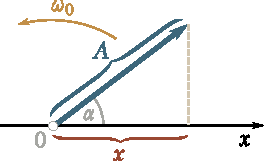
\includegraphics[scale=0.95]{figures/ch_07/fig_7_9.pdf}
		\caption[]{}
		\label{fig:7_9}
	\end{center}
\end{figure}

Ta hãy xét phép cộng hai đao động điều hòa cùng phương và cùng tần số. Độ đời $x$ của vật dao động sẽ là tổng các độ dời $x_1$ và $x_2$ được viết như sau:
\begin{equation}\label{eq:7_83}
	x_1 = A_1\cos(\omega_0 t + \alpha_1),\quad x_2 = A_2\cos(\omega_0 t + \alpha_2).
\end{equation}

\noindent
Ta biểu diễn cả hai dao động bằng các vector $\vec{A}_1$ và $\vec{A}_2$ (\fig{7_10}). Ta hãy về vector tổng hợp $\vec{A}$ theo các quy tắc cộng vector. Dễ dàng thấy rằng hình chiếu của vector này lên trục $x$ bằng tổng các hình chiếu của các vector số hạng:
\begin{equation*}
	x = x_1 + x_2.
\end{equation*}

\noindent
Do đó, vector $\vec{A}$ là dao động tổng hợp. Vector này quay với cùng vận tốc góc $\omega_0$, như các vector $\vec{A}_1$ và $\vec{A}_2$, cho nên chuyển động tổng hợp sẽ là một dao động điều hòa với tần số $\omega_0$, biên độ $A$ và pha ban đầu $\alpha$. Từ phép dựng rõ ràng là
\begin{align}
	A^2 &= A_1^2 + A_2^2 - 2A_1A_2\cos[\pi-(\alpha_2-\alpha_1)] \nonumber\\
	&= A_1^2 + A_2^2 - 2A_1A_2\cos(\alpha_2-\alpha_1), \label{eq:7_84}\\
	\tan\alpha &= \frac{A_1\sin\alpha_1 + A_2\sin\alpha_2}{A_1\cos\alpha_1 + A_2\cos\alpha_2}.\label{eq:7_85}
\end{align}

Vậy cách biểu diễn các dao động điều hòa trực tiếp bằng các vector cho khả năng quy phép cộng một số dao động về phép toán cộng các vector. Phương pháp này là đặc biệt có ích, chẳng hạn, trong quang học nơi mà dao động sáng tại một điểm nào đó được xác định như kết quả của sự chồng nhiều dao động đi tới điềm đã cho từ các phần khác nhau của mặt đầu sóng.

\begin{figure}[!htb]
	\begin{center}
		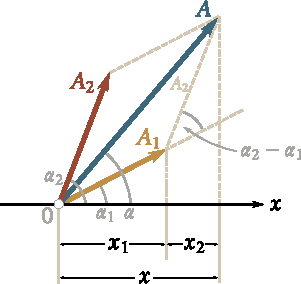
\includegraphics[scale=0.95]{figures/ch_07/fig_7_10.pdf}
		\caption[]{}
		\label{fig:7_10}
	\end{center}
\end{figure}

Có thể thu được, một cách hiển nhiên, các công thức~\eqref{eq:7_84} và~\eqref{eq:7_85} bằng cách cộng các biểu thức~\eqref{eq:7_83} và thực hiện các phép biến đổi lượng giác thích hợp. Nhưng cách mà ta đã áp dụng để thu được các công thức này có đặc điểm là rất đơn giản và dễ thấy.

Ta hãy phân tích biểu thức \eqn{7_84} của biên độ. Nếu hiệu pha của cả hai dao động $\alpha_2-\alpha_1$ là bằng không, thì biên độ của dao động tổng hợp bằng tổng $A_1$ và $A_2$. Nếu hiệu pha $\alpha_2-\alpha_1$ bằng $+\pi$ hay $-\pi$, nghĩa là cả hai dao động ngược pha nhau thì biên độ của dao động tổng hợp sẽ bằng $|A_1-A_2|$.

Nếu các tần số của các dao động $x_1$ và $x_2$ là không giống nhau thì các vector $\vec{A}_1$ và $\vec{A}_2$ sẽ quay với các vận tốc khác nhau. Trong trường hợp này vector tổng hợp $\vec{A}$ xung động về độ lớn và quay với vận tốc thay đổi. Do đó trong trường hợp này chuyển động tổng hợp sẽ không phải là một dao động điều hòa mà là một quá trình dao động phức tạp nào đó.

\section{Hiện tượng phách}\label{sec:7_8}

Một trường hợp có ý nghĩa đặc biệt là khi hai dao động điều hòa có tính cộng được có cùng phương, xấp xỉ nhau về tần số. Bây giờ ta sẽ chứng tỏ xem với những điều kiện này, khi nào có thể coi chuyển động tổng hợp như một dao động điều hòa với biên độ xung động. Một dao động như vậy được gọi là \textbf{phách}.

Ta ký hiệu tần số của một trong các dao động đó bằng chữ $\omega$, tần số của dao động thứ hai bằng $\omega+\Delta\omega$. Theo điều kiện $\Delta\omega\ll\omega$. Ta sẽ giả thử là các biên độ của cả hai dao động là như nhau và bằng $A$. Để không phức tạp hóa các công thức một cách không cần thiết, ta giả thử rằng các pha ban đầu của cả hai dao động đều bằng không. Khi đó các phương trình dao động sẽ có dạng sau:
\begin{equation*}
	x_1 = A\cos\omega t,\quad x_2 = A\cos(\omega+\Delta\omega) t.
\end{equation*}

\noindent
Cộng các biểu thức này và dùng công thức lượng giác cho tổng các cosine, ta được
\begin{equation}\label{eq:7_86}
	x = x_1 + x_2 = \left[ 2A \cos\left(\frac{\Delta\omega}{2}t\right)\right] \cos\omega t
\end{equation}

\noindent
(trong các thừa số thứ hai ta bỏ qua số hạng $\Delta\omega/2$ so với $\omega$). Đồ thị của hàm~\eqref{eq:7_86} được mô tả trên hình \fig{7_11}a. Đồ thị được vẽ đối với $\omega/\Delta\omega=10$.

\begin{figure}[!htb]
	\begin{minipage}[t]{\linewidth}
		\begin{center}
			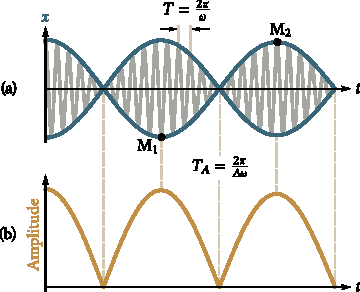
\includegraphics[scale=1.0]{figures/ch_07/fig_7_11.pdf}
			\caption[]{}
			\label{fig:7_11}
		\end{center}
	\end{minipage}
\end{figure}

Thừa số chứa trong dấu ngoặc công thức \eqn{7_86} biến đổi chậm hơn nhiều so với thừa số thứ hai. Do điều kiện $\Delta\omega\ll\omega$ nên trong khoảng thời gian mà thừa số $\cos\omega t$ thực hiện một số dao động toàn phần thì thừa số đứng trong các dấu ngoặc hầu như không thay đổi. Điều này cho ta cơ sở để coi dao động~\eqref{eq:7_86} như một dao động điều hòa có tần số $\omega$, có biên độ biến đổi theo một định luật tuần hoàn nào đó. Thừa số đứng trong các dấu ngoặc không thể là biểu thức của định luật này, vì nó biến đổi trong các phạm vi từ $-2A$ đến $+2A$ trong khi biên độ theo định nghĩa lại là một đại lượng dương. Đồ thị của biên độ được trình bày trên hình \fig{7_11}b. Rõ ràng là biểu thức giải tích của biên độ có dạng
\begin{equation}\label{eq:7_87}
	\text{amplitude} = \left|2A\cos\left(\frac{\Delta\omega}{2}t\right)\right|.
\end{equation}

\begin{figure}[!htb]
	\begin{minipage}[t]{\linewidth}
		\begin{center}
			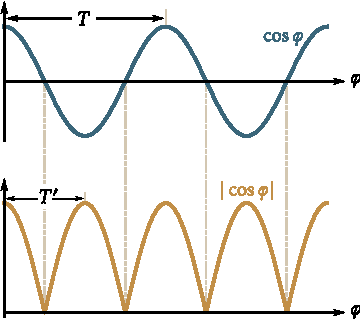
\includegraphics[scale=0.85]{figures/ch_07/fig_7_12.pdf}
			\caption[]{}
			\label{fig:7_12}
		\end{center}
	\end{minipage}
\end{figure}

Hàm~\eqref{eq:7_87} là hàm tuần hoàn với tần số lớn gấp $2$ lần tần số của biểu thức đứng dưới dấu module (xem hình \fig{7_12} trên đó ta dựng đồ thị của cosine và module của nó), nghĩa là với tần số $\Delta\omega$. Vậy tần số xung động của biên độ --- người ta gọi nó là tần số phách --- bằng hiệu các tần số của các dao động có cộng tính.

Ta chú ý rằng thừa số $2A\cos(\Delta\omega t/2)$ không chỉ xác định biên độ mà còn ảnh hưởng cả tới pha của dao động. Điều này biểu hiện, chẳng hạn, ở chỗ là các độ lệch ứng với các cực đại kề nhau của biên độ có các dấu ngược nhau (xem các điểm M$_1$ và M$_2$ trên hình \fig{7_11}a).

\section{Cộng các dao động vuông góc}\label{sec:7_9}

Ta giả thử rằng chất điểm có thể thực hiện các dao động dọc theo cả trục $x$ lẫn trục $y$ vuông góc với $x$. Nếu gây ra cả hai dao động, chất điểm sẽ chuyển động nói chung theo một quỹ đạo cong nào đó có dạng phụ thuộc vào hiệu các pha của cả hai dao động

Ta chọn gốc tính thời gian sao cho pha ban đầu của dao động thứ nhất là bằng không. Khi đó các phương trình dao động được viết như sau:
\begin{equation}\label{eq:7_88}
	x = A\cos\omega t,\quad y = B\cos(\omega t + \alpha)
\end{equation}

\noindent
trong đó $\alpha$ là hiệu các pha của cả hai dao động.

Các biểu thức~\eqref{eq:7_88} là phương trình được cho dưới dạng tham số của quỹ đạo mà theo đó vật chuyển động tham gia vào cả hai dao động. Để nhận được phương trình quỹ đạo dưới dạng thông thường, cần phải khử tham số $t$ khỏi các phương trình~\eqref{eq:7_88}. Từ phương trình~\eqref{eq:7_88} suy ra rằng
\begin{equation}\label{eq:7_89}
	\cos\omega t = \frac{x}{A}.
\end{equation}

\noindent
Do đó
\begin{equation}\label{eq:7_90}
	\sin\omega t = \left(1 - \frac{x^2}{A^2}\right)^{1/2}.
\end{equation}

\noindent
Bây giờ ta khai triển cosine ở phương trình thứ hai trong các phương trình~\eqref{eq:7_88} theo công thức đối với cosine của một tổng, đồng thời thay thế $\cos\omega t$ và $\sin\omega t$ bằng các giá trị~\eqref{eq:7_89} và~\eqref{eq:7_90} của chúng. Kết quả là ta được
\begin{equation*}
	\frac{y}{A} = \frac{x}{A}\cos\alpha - \sin\alpha \left(1 - \frac{x^2}{A^2}\right)^{1/2}.
\end{equation*}

\noindent
Sau các phép biến đổi đơn giản có thể đưa phương trình này về dạng
\begin{equation}\label{eq:7_91}
	\frac{x^2}{A^2} + \frac{y^2}{B^2} - \frac{2xy}{AB} \cos\alpha = \sin^2\alpha.
\end{equation}

Phương trình \eqn{7_91} nói chung, là phương trình của một đường elip có các trục được quay đối với các trục tọa độ $x$ và $y$. Sự định hướng của elip và độ lớn của các bán trục của nó phụ thuộc một cách khá phức tạp vào các biên độ $A$ và $B$ và hiệu các pha $\alpha$.

Ta xác định dạng quỹ đạo cho một số trường hợp đặc biệt.

\begin{figure}[!htb]
	\begin{minipage}[t]{0.5\linewidth}
		\begin{center}
			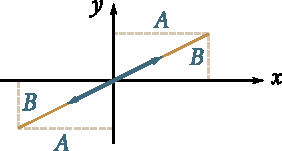
\includegraphics[scale=0.95]{figures/ch_07/fig_7_13.pdf}
			\caption[]{}
			\label{fig:7_13}
		\end{center}
	\end{minipage}
	\hspace{-0.0cm}
	\begin{minipage}[t]{0.5\linewidth}
		\begin{center}
			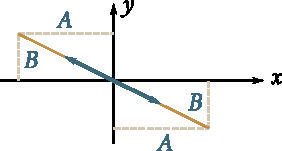
\includegraphics[scale=0.95]{figures/ch_07/fig_7_14.pdf}
			\caption[]{}
			\label{fig:7_14}
		\end{center}
	\end{minipage}
\end{figure}

\begin{enumerate}[1.]
	\item Hiệu các pha $\alpha$ là bằng không. Trong trường hợp này phương trình \eqn{7_91} có dạng
	\begin{equation*}
		\left(\frac{x}{A} - \frac{y}{B}\right)^{2} = 0
	\end{equation*}

	\noindent
	từ đó ta có được phương trình của đường thẳng:
	\begin{equation}\label{eq:7_92}
		y = \frac{B}{A}x.
	\end{equation}

	\noindent
	The oscillating particle moves along this straight line, its distance from the origin of coordinates being $r=\sqrt{x^2+y^2}$. Introducing into this equation the expressions~\eqref{eq:7_88} for $x$ and $y$ and taking into account that $a=0$, we get the law of the change in $r$ with time:
	\begin{equation}\label{eq:7_93}
		r = \left(x^2 + y^2\right)^{1/2}\cos\omega t.
	\end{equation}

	\noindent
	Từ \eqn{7_93} chuyển động tổng hợp là một dao động điều hòa dọc theo đường thẳng~\eqref{eq:7_92} với tần số $\omega$ và biên độ bằng $\sqrt{A^2+B^2}$ (\fig{7_13}).

	\item Hiệu các pha $\alpha$ bằng $\pm\pi$. Phương trình~\eqref{eq:7_91} có dạng
	\begin{equation*}
		\left(\frac{x}{A} + \frac{y}{B}\right)^{2} = 0
	\end{equation*}

	\noindent
	từ đó ta thu được chuyển động tổng hợp là một dao động điều hòa dọc theo đường thẳng (hình \fig{7_14}):
	\begin{equation*}
		y = -\frac{B}{A}x.
	\end{equation*}

	\item Với $\alpha=\pm\pi/2$ phương trình \eqn{7_91} chuyển thành
	\begin{equation}\label{eq:7_94}
		\frac{x^2}{A^2} + \frac{y^2}{B^2} = 1
	\end{equation}

	\noindent
	nghĩa là phương trình của một elip được quy về các trục tọa độ, thêm vào đó các bán trục của elip bằng các biên độ dao động tương ứng. Khi các biên độ $A$ và $B$ bằng nhau elip suy biến thành đường tròn.

	Các trường hợp $\alpha=+\pi/2$ và $\alpha=-\pi/2$ được phân biệt bằng chiều chuyển động trên elip hoặc trên đường tròn. Nếu $\alpha=+\pi/2$, có thể viết phương trình~\eqref{eq:7_88} như sau:
	\begin{equation}\label{eq:7_95}
		x = A\cos\omega t,\quad y = -B\sin\omega t.
	\end{equation}

	\noindent
	Tại thời điểm $t=0$ vật nằm tại điểm $1$ (hình \fig{7_15}). Tại các thời điểm sau tọa độ $x$ giảm, còn tọa độ $y$ là âm. Do đó chuyển động được thực hiện theo chiều kim đồng hồ.

	Với $\alpha=-\pi/2$ các phương trình dao động có dạng
	\begin{equation}\label{eq:7_96}
		x = A\cos\omega t,\quad y = B\sin\omega t.
	\end{equation}

	\noindent
	Từ đây có thể kết luận rằng chuyển động xảy ra ngược chiều kim đồng hồ.
\end{enumerate}

\begin{figure}[!htb]
	\begin{minipage}[t]{0.5\linewidth}
		\begin{center}
			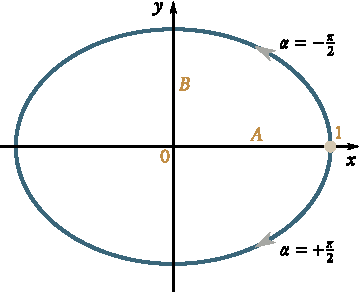
\includegraphics[scale=0.95]{figures/ch_07/fig_7_15.pdf}
			\caption[]{}
			\label{fig:7_15}
		\end{center}
	\end{minipage}
	\hspace{-0.0cm}
	\begin{minipage}[t]{0.5\linewidth}
		\begin{center}
			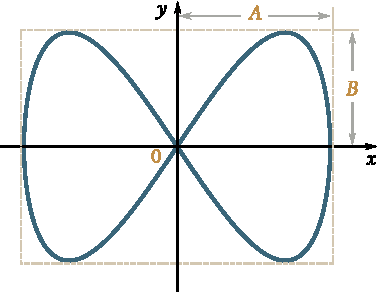
\includegraphics[scale=0.95]{figures/ch_07/fig_7_16.pdf}
			\caption[]{}
			\label{fig:7_16}
		\end{center}
	\end{minipage}
\end{figure}

Từ điều đã nói suy ra rằng chuyển động trên đường tròn có bán kính $R$ với vận tốc góc $\omega$ có thể được biểu diễn như tổng của hai dao động vuông góc:
\begin{equation}\label{eq:7_97}
	x = R\cos\omega t,\quad y = \pm R\sin\omega t
\end{equation}

\noindent
(dấu ``$+$'' trong biểu thức đối với $y$ ứng với chuyển động ngược chiều kim đồng hồ, dấu ``$-$'' ứng với chuyển động theo chiều kim đồng hồ).

Trong trường hợp khi các tần số của các dao động vuông góc khác nhau một lượng $\Delta\omega$ rất bé thì có thể coi chúng như các dao động có tần số như nhau nhưng với hiệu các pha biến đổi chậm. Thực vậy, có thể biểu diễn các phương trình dao động như sau:
\begin{equation*}
	x = A\cos\omega t,\quad y = B\cos[\omega t + (\Delta\omega t + \alpha)]
\end{equation*}

\noindent
và coi biểu thức $\Delta\omega t + \alpha$ như hiệu các pha biến đổi chậm với thời gian theo định luật tuyến tính.

Chuyển động tổng hợp trong trường hợp này xảy ra theo một đường cong có hình dạng biến đổi chậm; đường cong đó liên tục có dạng thỏa mãn mọi giá trị của hiệu các pha từ $-\pi$ đến $+\pi$.

Nếu các tần số của các dao động vuông góc với nhau là khác nhau thì quỹ đạo của chuyển động tổng hợp có dạng các đường cong khá phức tạp được gọi là các \textbf{hình Lissajous}. Trên hình~\ref{fig:7_16} trình bày một trong các quỹ đạo đơn giản nhất thu được với tỷ số của các tần số là $1$:$2$ và hiệu các pha là $\pi/2$. Các phương trình dao động có dạng
\begin{equation*}
	x = A\cos\omega t,\quad y = B\cos\left(\omega t + \frac{\pi}{2}\right).
\end{equation*}

\noindent
Trong khi mà dọc theo trục $x$ một điểm có thể dịch chuyển từ vị trí biên này tới vị trí biên kia, dọc theo trục $y$ nếu nó đi khỏi vị trí không, thì nó có thể đạt tới một vị trí biên này, sau đó tới vị trí biên kia và trở về vị trí không.

Với tỷ số các tần số là $1$:$2$ và hiệu các pha bằng không, quỹ đạo sẽ suy biến thành một đường cong không kín (hình \fig{7_17}) mà trên đó điểm chuyển động cả đi lẫn về.

\begin{figure}[!htb]
	\begin{minipage}[t]{0.5\linewidth}
		\begin{center}
			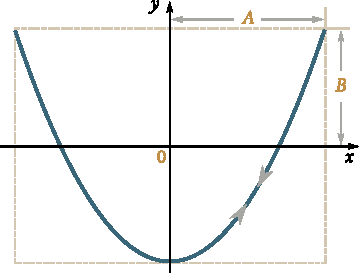
\includegraphics[scale=0.95]{figures/ch_07/fig_7_17.pdf}
			\caption[]{}
			\label{fig:7_17}
		\end{center}
	\end{minipage}
	\hspace{-0.05cm}
	\begin{minipage}[t]{0.5\linewidth}
		\begin{center}
			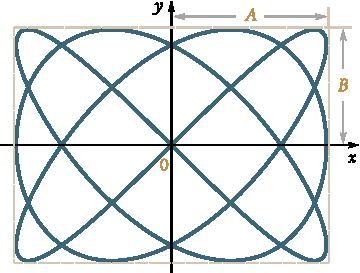
\includegraphics[scale=0.95]{figures/ch_07/fig_7_18.pdf}
			\caption[]{}
			\label{fig:7_18}
		\end{center}
	\end{minipage}
\end{figure}

Phân số hữu tỷ biểu thị tỷ số các tần số dao động càng gần tới đơn vị thì hình Lissajous càng trở nên phức tạp hơn. Trên hình~\ref{fig:7_18} để làm ví dụ ta trình bày đường cong đối với tỷ số các tần số là $3$:$4$ và hiệu các pha là $\pi/2$.

\section{Dao động tắt dần}\label{sec:7_10}

Dao động tắt dần được miêu tả bằng \eqn{7_11}:
\begin{equation*}
	\ddot{x} + 2\beta\dot{x} + \omega_0^2 x = 0
\end{equation*}

\noindent
trong đó~\eqref{eq:7_10} và~\eqref{eq:7_6},
\begin{equation*}
	2\beta = \frac{r}{m},\quad \omega_0^2 = \frac{k}{m}.
\end{equation*}

\noindent
Ở đây $r$ là hệ số cản, nghĩa là hệ số tỷ lệ giữa vận tốc $\dot{x}$ và lực cản; $k$ là hệ số lực giả đàn hồi. Ta chú ý rằng $\omega_0$ là tần số mà các dao động tự do của hệ khi không có sự cản của môi trường (khi $r=0$) đã thực hiện. Người ta gọi tần số này là \textbf{tần số riêng} của hệ.

Việc thay hàm $x=e^{\lambda t}$ vào \eqn{7_11} sẽ dẫn tới phương trình đặc trưng
\begin{equation}\label{eq:7_98}
	\lambda^2 + 2\beta\lambda + \omega_0^2 = 0.
\end{equation}

\noindent
Các nghiệm của phương trình này bằng
\begin{equation}\label{eq:7_99}
	\lambda_1 = -\beta + \left(\beta^2 - \omega_0^2\right)^{1/2},\quad \lambda_2 = -\beta - \left(\beta^2 - \omega_0^2\right)^{1/2}.
\end{equation}

Với sự tắt dần không quá lớn (với $\beta<\omega_0$) thì biểu thức dưới dấu căn sẽ là âm. Ta biểu diễn nó dưới dạng $(i\omega)^2$, trong đó $\omega$ là đại lượng thực bằng
\begin{equation}\label{eq:7_100}
	\omega = \left(\omega_0^2 - \beta^2\right)^{1/2}.
\end{equation}

\noindent
Khi đó các nghiệm của phương trình đặc trưng được viết như sau:
\begin{equation}\label{eq:7_101}
	\lambda_1 = -\beta + i\omega,\quad \lambda_2 = -\beta - i\omega.
\end{equation}

Theo \eqn{7_38} nghiệm tổng quát của \eqn{7_11} là hàm
\begin{equation*}
	x = C_1e^{(-\beta + i\omega)t} + C_2e^{(-\beta - i\omega)t} = e^{\beta t} \left(C_1e^{i\omega t} + C_2e^{-i\omega t}\right).
\end{equation*}

\noindent
Biểu thức trong các dấu ngoặc tương tự như \eqn{7_51}. Do đó có thể biểu diễn nó dưới dạng tương tự \eqn{7_55}. Vậy với sự tắt dần không quá mạnh nghiệm tổng quát của phương trình \eqn{7_11} có dạng
\begin{equation}\label{eq:7_102}
	x = A_0 e^{\beta t} \cos(\omega t + \alpha).
\end{equation}

\noindent
Ở đây $A_0$ và $\alpha$ là các hằng số tùy ỳ, $\omega$ là đại lượng được xác định bằng công thức \eqn{7_100}. Trên hình~\ref{fig:7_19} người ta cho đồ thị của hàm~\eqref{eq:7_102}. Các giới hạn mà độ dời $x$ của điểm dao động nằm trong đó được vẽ bằng các đường chấm chấm.

Ứng với dạng hàm~\eqref{eq:7_102} có thể coi chuyển động của hệ như một dao động điều hòa có tần số $\omega$ với biên độ biến thiên theo định luật $A(t)=A_0e^{-\beta t}$. Trên hình \fig{7_19} đường cong chấm chấm phía trên cho đồ thị của hàm $A(t)$, thêm vào đó đại lượng $A_0$ là biên độ tại thời điểm ban đầu. Ngoài $A_0$ ra độ dời ban đầu $x_0$ cũng phụ thuộc vào pha ban đầu $\alpha$: $x_0=A_0\cos\alpha$.

\begin{figure}[!htb]
	\begin{center}
		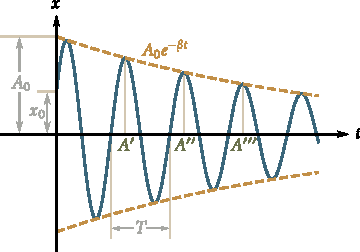
\includegraphics[scale=1.0]{figures/ch_07/fig_7_19.pdf}
		\caption[]{}
		\label{fig:7_19}
	\end{center}
\end{figure}

Vận tốc của sự tắt dần của dao động được xác định bằng đại lượng $\beta=r/(2m)$ mà người ta gọi là \textbf{hệ số tắt dần}. Ta tìm thời gian $\tau$ mà biên độ giảm $e$ lần. Theo định nghĩa $e^{-\beta\tau}=e^{-1}$ từ đó $\beta\tau=1$. Do đó, hệ số tắt dần, về độ lớn, là nghịch đảo với khoảng thời gian mà biên độ giảm $e$ lần.

Theo công thức \eqn{7_56} chu kỳ của dao động tắt dần bằng
\begin{equation}\label{eq:7_103}
	T = \frac{2\pi}{\left(\omega_0^2 - \beta^2\right)^{1/2}}.
\end{equation}

\noindent
Với sự cản không lớn của môi trường $(\beta^2 \ll \omega_0^2)$ chu kỳ dao động thực tế bằng $T_0=2\pi/\omega_0$. Với sự tăng của hệ số tắt dần chu kỳ dao động sẽ tăng lên.

Các độ lệch lớn nhất liên tiếp nhau về một phía bất kỳ nào đó (chẳng hạn $A', A'', A'''$, v.v... trên hình \fig{7_19}) tạo thành một cấp số nhân. Thực vậy, nếu $A'=A_0e^{-\beta t}$ thì $A''=A_0e^{-\beta(t+T)}=A'e^{-\beta T}$, $A'''=A_0e^{[-\beta(t+2T)]}=A''e^{-\beta T}$, v.v... Nói chung tỷ số giữa các giá trị của các biên độ ứng với các thời điểm khác nhau một chu kỳ là bằng
\begin{equation*}
	\frac{A(t)}{A(t+T)} = e^{\beta T}.
\end{equation*}

\noindent
Người ta gọi tỷ số này là \textbf{giảm lượng tắt dần}, còn loga của nó là  \textbf{giảm lượng loga tắt dần}:
\begin{equation}\label{eq:7_104}
	\lambda = \ln\left[\frac{A(t)}{A(t+T)}\right] = \beta T
\end{equation}

\noindent
[không nên lẫn lộn với $\lambda$ trong các công thức\eqref{eq:7_98} và~\eqref{eq:7_101}].

Để đặc trưng cho hệ dao động người ta thường dùng giảm lượng loga tắt dần $\lambda$. Theo \eqn{7_104} nếu biểu thị $\beta$ qua $\lambda$ và $T$ có thể viết định luật sự giảm biên độ với thời gian dưới dạng
\begin{equation}\label{eq:7_105}
	A = A_0\exp\left(-\frac{\lambda}{T}\,t\right).
\end{equation}

\noindent
Trong thời gian $\tau$ mà biên độ giảm $e$ lần, hệ sẽ kịp thực hiện $N_e=\tau/T$ dao động. Từ điều kiện $\exp(-\lambda t/T)=\exp(-1)$ ta thu được là $\lambda t/T=1$. Do đó, giảm lượng loga tắt dần về độ lớn là nghịch đảo với số dao động thực hiện được trong thời gian mà biên độ giảm $e$ lần.

Để đặc trưng cho hệ dao động người ta cũng thường sử dụng đại lượng
\begin{equation}\label{eq:7_106}
	Q = \frac{\pi}{\lambda} = \pi N_e
\end{equation}

\noindent
được gọi là \textbf{hệ số phẩm chất} của hệ dao đông. Như đã thấy từ định nghĩa của nó, hệ số phẩm chất tỷ lệ với số dao động $N_e$ do hệ thực hiện được trong thời gian $\tau$ mà biên độ dao động giảm $e$ lần.

We established in Sec.~\ref{sec:7_5} that the total energy of an oscillating system is proportional to the square of the amplitude [see \eqn{7_68}]. Accordingly, the energy of the system in damped oscillations diminishes with time according to the law
\begin{equation}\label{eq:7_107}
	E = E_0 e^{-2\beta t}
\end{equation}

\noindent
($E_0$ is the value of the energy at $t=0$). Time differentiation of this expression gives the rate of growth of the system's energy:
\begin{equation*}
	\diff{E}{t} = -2\beta E_0 e^{-2\beta t} = -2\beta E.
\end{equation*}

\noindent
Đổi dẫu ngược lại, ta tìm được tốc độ của sự giảm năng lượng:
\begin{equation}\label{eq:7_108}
	-\diff{E}{t} = 2\beta E.
\end{equation}

\noindent
Nếu năng lượng biến đổi ít trong một khoảng thời gian bằng chu kỳ dao động thì có thể tìm được độ giảm năng lượng bằng cách nhân biểu thức \eqn{7_108} với $T$:
\begin{equation*}
	-\Delta E = 2\beta T E
\end{equation*}

\noindent
(ta nhớ rằng $\Delta E$ ký hiệu cho số gia, còn $-\Delta E$ là độ giảm năng lượng). Cuối cùng, chú ý tới các công thức~\eqref{eq:7_104} và~\eqref{eq:7_106} ta sẽ đi tới hệ thức
\begin{equation}\label{eq:7_109}
	\frac{E}{(-\Delta E)} = \frac{Q}{2\pi}
\end{equation}

\noindent
từ đó suy ra rằng, với sự tắt dần yếu của các dao động, hệ số phẩm chất vơi độ chính xác đến thừa số $2\pi$ là bằng tỷ số năng lượng được dự trự trong hệ tại thời điểm đã cho với độ giảm của năng lượng này trong một chu kỳ dao động.

\begin{figure}[!htbt]
	\begin{center}
		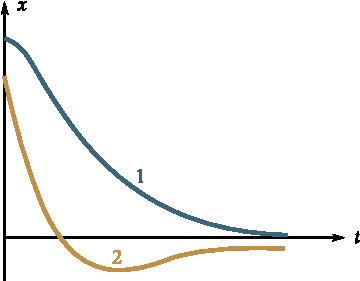
\includegraphics[scale=0.95]{figures/ch_07/fig_7_20.pdf}
		\caption[]{}
		\label{fig:7_20}
	\end{center}
	\vspace{-0.8cm}
\end{figure}

Từ công thức \eqn{7_103} suy ra rằng với sự tăng của hệ số tắt dần chu kỳ dao động cũng tăng lên. Khi $\beta=\omega_0$ chu kỳ dao động trở thành vô cùng, nghĩa là chuyển động sẽ là tuần hoàn.

Khi $\beta>\omega_0$ các nghiệm của phương trình đặc trưng là các nghiệm thực [xem \eqn{7_99}] và nghiệm của phương trình vi phân~\eqref{eq:7_11} bằng tổng của hai hàm mũ:
\begin{equation*}
	x = C_1e^{-\lambda_1 t} + C_2e^{-\lambda_2 t}.
\end{equation*}

\noindent
Ở đây $C_1$ và $C_2$ là các hằng số thực có các giá trị phụ thuộc vào các điều kiện ban đầu (vào $x_0$ và $v_0=\dot{x}_0$). Do đó, chuyển động mang tính chất không tuần hoàn (không có chu kỳ), nghĩa là nếu bị đẩy ra khỏi vị trí cân bằng hệ sẽ trở về vị trí cân bằng mà không thực hiện các dao động. Trên hình~\ref{fig:7_20} người ta trình bà hai cách mà hệ có thể trở về vị trí cân bằng trong chuyển động không tuần hoàn. Bằng cách nào đó trong các cách đó để hệ trở về vị trí cân bằng là tùy thuộc vào các điều kiện ban đầu. Chuyển động được mô tả bằng đường cong $2$ thu được trong trường hợp khi hệ bắt đầu chuyển động từ vị trí đặc trưng bởi độ dời $x_0$ về vị trí cân bằng với vận tốc ban đầu $v_0$ xác định bởi điều kiện
\begin{equation}\label{eq:7_110}
	|v_0| > |x_0|\left[\beta + \left(\beta^2 + \omega_0^2\right)^{1/2}\right].
\end{equation}

\noindent
Điều kiện này sẽ được thực hiện trong trường hợp nếu truyền một va đập khá mạnh về vị trí cân bằng cho một hệ đã bị đẩy khỏi vị trí cân bằng. Nếu đưa hệ khỏi vị trí cân bằng rồi buông ra mà không va đập vào nó (nghĩa là với $v_0=0$) hoặc truyền cho nó một va đập không đủ mạnh [sao cho $v_0$ là nhỏ hơn giá trị xác định bởi~\eqref{eq:7_110}], thì chuyển động sẽ xảy ra ứng với đường cong $1$ trên hình \fig{7_20}.

\section{Tự dao động}\label{sec:7_11}

Trong các dao động tắt dần năng lượng của hệ được chi phí để thắng sự cẳn của môi trường. Nếu bù lại sự giảm năng lượng này thì dao động trở thành dao động không tắt. Sự bù năng lượng này cho hệ có thể được thực hiện do các va đập từ bên ngoài, tuy nhiên các va đập này phải được truyền cho hệ đúng nhịp với các dao động của hệ, trong trường hợp ngược lại chúng có thể làm yếu các dao động và thậm chí làm ngừng hoàn toàn các dao động. Có thể làm sao cho hệ dao động tự điều khiển tác động bên ngoài bằng cách đảm bảo sự phối hợp chặt chẽ các va đập truyền cho hệ với chuyển động của hệ. Một hệ như vậy được gọi là một \textbf{hệ tự dao động}, và các dao động không tắt mà hệ thực hiện là các \textbf{tự dao động}.

\begin{figure}[!htb]
	\begin{center}
		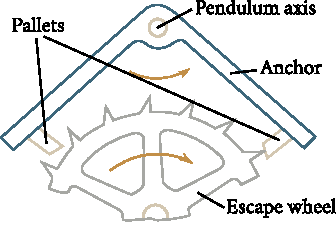
\includegraphics[scale=0.95]{figures/ch_07/fig_7_21.pdf}
		\caption[]{}
		\label{fig:7_21}
	\end{center}
\end{figure}

Để làm ví dụ về một hệ tự dao động, ta xét một cơ cấu đồng hồ. Con lắc đồng hồ được cắm vào một trục có tay đòn uốn cong, nghĩa là một cái móc neo (\fig{7_11}). Tại các đầu của móc neo có các chỗ nhô ra có hình dạng đặc biệt được gọi là các palet. Bánh xe răng cưa dẫn động chịu tác động của một dây xích có quả nặng hoặc của một lò xo bị xoắn mà chúng muốn quay bánh xe theo chiều kim đồng hồ. Tuy nhiên một phần lớn thời gian bánh xe tì một trong các răng vào mặt bên của một palet nào đó trượt theo bề mặt của răng khi con lắc đu đưa. Chỉ vào lúc mà con lắc ở gần vị trí cân bằng các palet mới thôi không chặn đường các răng nữa và bánh xe dẫn động sẽ quay do một răng trượt cái đỉnh của nó theo mặt vát của palet khi đụng vào cái móc neo. Trong một vòng đu đưa toàn phần của con lắc (trong một chu kỳ) bánh xe dẫn động quay được hai răng, trong khi đó mỗi palet nhận được từng va đập một. Sự giảm năng lượng của con lắc xuất hiện do ma sát sẽ được bổ sung bằng năng lượng của quả nặng được nâng lên hoặc của lò xo bị xoắn thông qua các va đập này.

\section{Dao động cưỡng bức}\label{sec:7_12}

Trong trường hợp khi lực cưỡng bức biến đổi theo một định luật điều hòa, dao động sẽ được mô tả bằng phương trình vi phân:
\begin{equation}\label{eq:7_111}
	\ddot{x} + 2\beta\dot{x} + \omega_0^2 x = f_0\cos\omega t
\end{equation}

\noindent
[xem \eqn{7_13}]. Ở đây $\beta$ là hệ số tắt dần, $\omega_0$ là tần số riêng của hệ [xem~\eqref{eq:7_6}, \eqref{eq:7_10}], $f_0=F_0/m$ ($F_0$ là biên độ của lực cưỡng bức), $\omega$ là tần số của lực.

Phương trình~\eqref{eq:7_111} là phương trình không thuần nhất. Theo định lý~\eqref{eq:7_41} nghiệm tổng quát của phương trình không thuần nhất bằng tổng của nghiệm tổng quát của phương trình thuần nhất tương ứng và một nghiệm riêng của phương trình không thuần nhất. Chúng ta đã biết nghiệm tổng quát của phương trình thuần nhất [xem~\eqref{eq:7_102}, là nghiệm tổng quát của \eqn{7_11}]. Nó có dạng
\begin{equation}\label{eq:7_112}
	x = A e^{-\beta t} \cos(\omega' t + \alpha)
\end{equation}

\noindent
trong đó $\omega'=\left(\omega_0^2 - \beta^2\right)^{1/2}$, còn $A_0$ và $\alpha$ là các hằng số tùy ý\footnote{Ta đã ký hiệu tần số lực cưỡng bức bằng chữ $\omega$ không có dấy phẩy}.

Còn phải tìm nghiệm riêng (không chứa các hằng số tùy ý) của phương trình \eqn{7_111}. Muốn vậy ta sử dụng thủ thuật đã được mô tả ở cuối~\ref{sec:7_4}. Ta thêm vào hàm ở vế phải của phương trình \eqn{7_111} một hàm ảo $if_0\sin\omega t$, sau đó biểu diễn vế phải dưới dạng $f_0\exp(i\omega t)$ [xem \eqn{7_24}]. Như vậy ta đi tới phương trình:
\begin{equation}\label{eq:7_113}
	\ddot{x} + 2\beta\dot{x} + \omega_0^2 x = f_0 e^{i\omega t}.
\end{equation}

\noindent
Giải phương trình này dễ hơn giải phương trình \eqn{7_111}, vì lấy vi phân và tích phân hàm mũ đơn giản hơn là các hàm lượng giác.

Ta thử nghiệm riêng của phương trình \eqn{7_113} dưới dạng
\begin{equation}\label{eq:7_114}
	\hat{x} = \hat{A} e^{i\omega t}
\end{equation}

\noindent
trong đó $\hat{A}$ là một số phức nào đó. Hàm~\eqref{eq:7_114} cũng là hàm phức nên được đánh dấu bằng dẫu mũ trên $x$. Lấy vi phân hàm này theo t ta được:
\begin{equation}\label{eq:7_115}
	\diff{\hat{x}}{t} = i\omega \hat{A} e^{i\omega t},\quad \diffsec{\hat{x}}{t} = -\omega^2 \hat{A} e^{i\omega t}.
\end{equation}

\noindent
Thế các biểu thức~\eqref{eq:7_114} và~\eqref{eq:7_115} vào phương trình \eqn{7_113} và sau khi ước lược thừa số chung $e^{i\omega t}$ sẽ dẫn tới phương trình đại số:
\begin{equation*}
	- \omega^2 \hat{A} + 2i\beta\omega\hat{A} + \omega^2\hat{A} = f_0.
\end{equation*}

\noindent
Từ đó
\begin{equation}\label{eq:7_116}
	\hat{A} = \frac{f_0}{\left(\omega_0^2 - \omega^2\right) + 2i\beta\omega}.
\end{equation}

\noindent
Ta tìm được giá trị của $\hat{A}$ mà hàm~\eqref{eq:7_114} thỏa mãn phương trình \eqn{7_113}. Ta biểu diễn số phức ở mẫu số dưới dạng số mũ:
\begin{equation}\label{eq:7_117}
	\left(\omega_0^2 - \omega^2\right) + 2i\beta\omega = \rho e^{i\varphi}.
\end{equation}

\noindent
Theo các công thức~\eqref{eq:7_18}
\begin{equation}\label{eq:7_118}
	\rho = \left[\left(\omega_0^2 - \omega^2\right)^2 + 4\beta^2\omega^2\right],\quad  \varphi = \arctan\left(\frac{2\beta\omega}{\omega_0^2 - \omega^2}\right).
\end{equation}

Thay thế mẫu số ứng với \eqn{7_117} vào \eqn{7_116} sẽ cho
\begin{equation*}
	\hat{A} = \frac{f_0}{\rho e^{i\varphi}} = \frac{f_0}{\rho}e^{-i\varphi}.
\end{equation*}

\noindent
Thay thế giá trị này của $\hat{A}$ vào~\eqref{eq:7_114}, ta được nghiệm riêng của phương trình \eqn{7_113}:
\begin{equation*}
	\hat{x} = \frac{f_0}{\rho} e^{-i\varphi} e^{i\omega t} = \frac{f_0}{\rho} e^{i(\omega t-\varphi)}.
\end{equation*}

\noindent
Cuối cùng, lấy phần thực của hàm này ta thu được nghiệm riêng của phương trình \eqn{7_111}:
\begin{equation*}
	x = \frac{f_0}{\rho} \cos(\omega t-\varphi).
\end{equation*}

\noindent
Thế giá trị $f_0$ và cả các giá trị~\eqref{eq:7_118} đối với $\rho$ và $\varphi$ sẽ dẫn tới biểu thức cuối cùng:
\begin{equation}\label{eq:7_119}
	x = \frac{F_0/m}{\left[\left(\omega_0^2 - \omega^2\right)^2 + 4\beta^2\omega^2\right]}\cos\left[\omega t - \arctan\left(\frac{2\beta\omega}{\omega_0^2 - \omega^2}\right)\right].
\end{equation}

\noindent
Ta chú ý rằng hàm~\eqref{eq:7_119} không chứa các hằng số tùy ý.

Ta thu được nghiệm riêng của phương trình \eqn{7_111} bằng một cách nữa nghĩa là nhờ giản đồ vector. Ta giả thử rằng nghiệm riêng của phương trình \eqn{7_111} có dạng
\begin{equation}\label{eq:7_120}
	x = A\cos(\omega t - \varphi).
\end{equation}

\noindent
Khi đó
\begin{align}
	\dot{x} &= -\omega A\sin(\omega t - \varphi) = \omega A\cos\left(\omega t - \varphi + \frac{\pi}{2}\right)\label{eq:7_121}\\
	\ddot{x} &= \omega^2 A\cos(\omega t - \varphi) = \omega^2 A\cos(\omega t - \varphi + \pi)\label{eq:7_122}.
\end{align}

\noindent
Thế các biểu thức~\eqref{eq:7_120}-\eqref{eq:7_122} vào \eqn{7_111} sẽ dẫn tới hệ thức
\begin{equation}\label{eq:7_123}
	\omega^2 A\cos(\omega t - \varphi + \pi) + 2\beta\omega A \cos\left(\omega t - \varphi + \frac{\pi}{2}\right) +
	\omega^2 A\cos(\omega t - \varphi) = f_0\cos\omega t.
\end{equation}

\begin{figure}[t]
	\begin{center}
		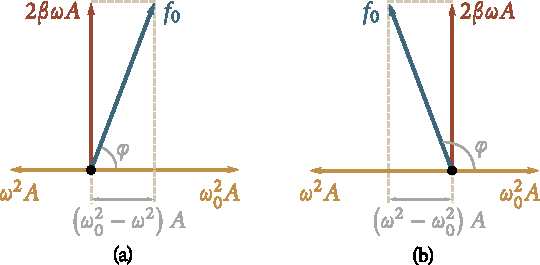
\includegraphics[scale=0.95]{figures/ch_07/fig_7_22.pdf}
		\caption[]{}
		\label{fig:7_22}
	\end{center}
	\vspace{-0.8cm}
\end{figure}

Từ \eqn{7_123} suy ra rằng các hắng số $A$ và $\varphi$ phải có các giá trị sao cho hàm điều hòa $f_0\cos\omega t$ là bằng tổng của ba hàm điều hòa ở vế trái của phương trình. Nếu mô tả hàm $\omega_0^2A\cos(\omega t-\varphi)$ bằng vector có độ dài $\omega_0^2A$ hướng về bên phải thì hàm $2\beta\omega A\cos(\omega t-\varphi+\pi/2)$ được mô tả bằng vector có độ dài $2\beta\omega A$ (hình \fig{7_22}) quay ngược chiều kim đồng hồ một góc $\pi/2$ đối với vector $\omega_0^2A$ (xem~\ref{sec:7_7}), còn hàm $\omega^2A\cos(\omega t-\varphi+\pi)$ được biểu diễn bằng vector có độ dài $\omega_0^2A$ quay một góc $\pi$ đối với vector $\omega_0^2A$. Để phương trình \eqn{7_123} được thỏa mãn thì tổng của ba vector kể trên phải trùng với vector mô tả hàm $f_0\cos\omega t$. Từ hình \fig{7_22}a rõ ràng là sự trùng nhau như vậy chỉ có thể xảy ra với giá trị biên độ $A$ được xác định bằng điều kiện:
\begin{equation*}
	\left(\omega_0^2 - \omega^2\right)^2A^2 + 4\beta^2\omega^2A^2 = f_0^2
\end{equation*}

\noindent
từ đó
\begin{equation}\label{eq:7_124}
	A = \frac{F_0/m}{\left[\left(\omega_0^2 - \omega^2\right)^2 + 4\beta^2\omega^2\right]}
\end{equation}

\noindent
(ta đã thay thế $f_0$ bằng tỷ số $F_0/m$). Hình~\ref{fig:7_22}a ứng với trường hợp $\omega<\omega_0$. Từ hình \fig{7_22}b ứng với trường hợp $\omega>\omega_0$ ta được cùng giá trị như vậy của $A$.

Hình~\ref{fig:7_22} cũng cho phép thu được cả giá trị của $\varphi$ là trị số của độ chậm pha của dao động cưỡng bức~\eqref{eq:7_120} so với lực cưỡng bức đã gây ra nó. Từ hình vẽ suy ra rằng
\begin{equation}\label{eq:7_125}
	\tan\varphi = \frac{2\beta\omega}{\omega_0^2 - \omega^2}.
\end{equation}

\noindent
Thay các giá trị $A$ và $\varphi$ được xác định bằng các công thức~\eqref{eq:7_124} và~\eqref{eq:7_125} vào \eqn{7_120} ta được hàm~\eqref{eq:7_119}.

Hàm~\eqref{eq:7_119} cộng với \eqn{7_112} cho nghiệm tổng quát của phương trình \eqn{7_111} mô tả hành trạng của hệ trong dao động cưỡng bức. Số hạng~\eqref{eq:7_112} có vai trò rõ rệt chỉ trong giai đoạn đầu của quá trình khi thiết lập dao động ( hình \fig{7_23}). Do có thừa số $e^{-\beta t}$ nên vai trò của số hạng~\eqref{eq:7_112}  bị giảm nhiều nhất với thời gian, và sau một thời gian vừa đủ có thể bỏ qua nó bằng cách chỉ giữ lại trong nghiệm số hạng~\eqref{eq:7_119}.

\begin{figure}[!htb]
	\begin{center}
		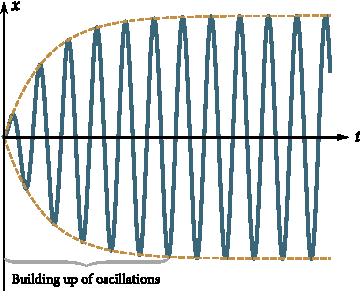
\includegraphics[scale=0.95]{figures/ch_07/fig_7_23.pdf}
		\caption[]{}
		\label{fig:7_23}
	\end{center}
	\vspace{-0.8cm}
\end{figure}

Vậy hàm~\eqref{eq:7_119} mô tả dao động cưỡng bức được thiết lập. Nó là dao động điều hòa với tần số bằng tần số của lực cưỡng bức. Biên độ~\eqref{eq:7_124} của dao động cưỡng bức tỷ lệ với biên độ của lực cưỡng bức. Đối với một hệ dao động đã cho (có các $\omega_0$ và $\beta$ xác định) biên độ phụ thuộc vào tần số của lực cưỡng bức. Dao động cưỡng bức chậm pha so với lực cưỡng bức, trong khi đó trị số của độ chậm $\varphi$ cũng phụ thuộc vào tần số của lực cưỡng bức [xem \eqn{7_125}].

Sự phụ thuộc của biên độ dao động cưỡng bức vào tần số của lực cưỡng bức dẫn tới điều là với một tần số xác định nào đó đối với một hệ đã cho biên độ dao động sẽ đạt giá trị cực đại. Hệ dao động sẽ đặc biệt hưởng ứng sự tác dụng cảu lực cưỡng bức ở tần số này. Hiện tượng này được gọi là \textbf{sự cộng hưởng}, còn tần số tương ứng là \textbf{tần số cộng hưởng}.

Để xác định tần số cộng hưởng $\omega_{\text{c}}$ cần phải tìm cực đại của hàm~\eqref{eq:7_124} hay cũng chính là cực tiểu của biểu thức dưới dấu căn ở mẫu số/ Lấy vi phân biểu thức đó theo $\omega$ và cho bằng không ta được điều kiện xác định $\omega_{\text{c}}$:
\begin{equation}\label{eq:7_126}
	-4\left(\omega_0^2 - \omega^2\right)\omega + 8\beta^2\omega = 0.
\end{equation}

Phương trình~\eqref{eq:7_126} có ba nghiệm: $\omega=0$ và
$\omega=\pm\left(\omega_0^2-2\beta^2\right)^{1/2}$. Nghiệm bằng không ứng với cực đại của mẫu số. Trong hai nghiệm còn lại phải bỏ nghiệm âm đi vì nó không có ý nghĩa vật lý (tần số không thể là âm). Vậy ta thu được một giá trị cho tần số cộng hưởng:
\begin{equation}\label{eq:7_127}
	\omega_{\text{c}} = \left(\omega_0^2-2\beta^2\right)^{1/2}.
\end{equation}

\noindent
Thay giá trị này của tần số vào \eqn{7_124} ta được biểu thức cho biên độ khi cộng hưởng
\begin{equation}\label{eq:7_128}
	A_{\text{c}} = \frac{F_0/m}{2\beta \left( \omega_0^2 - \beta^2\right)^{1/2}}.
\end{equation}

\noindent
Từ \eqn{7_128} suy ra rằng, khi không có sự cản của môi trường biên độ khi cộng hưởng biến thành vô cùng. Theo \eqn{7_127} tần số cộng hưởng trong chính các điều kiện này (khi $\beta=0$) sẽ trùng với tần số dao động riêng của $\omega_0$ của hệ.

Sự phụ thuộc của biên độ dao động cưỡng bức vào tần số của lực cưỡng bức (hay cũng chính là vào tần số dao động) được trình bày bằng đồ thị trên hình \fig{7_24}. Các đường cong riêng biệt trên đồ thị ứng với các giá trị khác nhau của tham số $\beta$. Theo~\eqref{eq:7_127} và~\eqref{eq:7_128} nếu $\beta$ càng nhỏ thì cực đại của đường cong đã cho nằm càng cao và càng sang bên phải. Với sự tắt dần rất lớn (sao cho $2\beta^2>\omega_0^2$) biểu thức đối với tần số cộng hưởng là ảo. Điều này có nghĩa là trong các điều kiện này sự cộng hưởng không quan sát được, nghĩa là với sự tăng của tần số, biên độ dao động cưỡng bức giảm đơn điệu (xem đường cong dưới cùng trên hình \fig{7_24}). Tập hợp các đồ thị khác nhau của hàm \fig{7_24} được mô tả trên hình \fig{7_24} ứng với các giá trị khác nhau của tham số $\beta$ được gọi là các \textbf{đường cong cộng hưởng}.

\begin{figure}[!htb]
	\begin{center}
		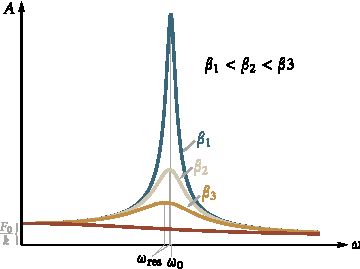
\includegraphics[scale=0.95]{figures/ch_07/fig_7_24.pdf}
		\caption[]{}
		\label{fig:7_24}
	\end{center}
\end{figure}

Về các đường cong cộng hưởng còn có thể cho nhận xét như sau. Khi $\omega$ tiến tới không tất cả các đường cong đi tới cùng một giá trị giới khác không bằng $F_0/(m\omega_0^2)$, nghĩa là $F_0/k$. Giá trị này là độ dời khỏi vị trí cân bằng mà hệ nhận được dưới tác dụng của một lực không đổi có độ lớn là $F_0$. Khi $\omega$ tiến tới vô cùng tất cả các đường cong sẽ tiệm cận tới không, vì với tần số lớn lực sẽ đổi chiều nhanh chóng sao cho hệ không kịp rời khỏi vị trí cân bằng một cách đáng kể. Cuối cùng ta chú ý rằng $\beta$ càng nhỏ thì biên độ gần cộng hưởng bị biến đổi càng nhanh với tần số và ta được cực đại càng ``nhọn''.

Từ công thức \eqn{7_128} suy ra rằng khi sự tắt dần nhỏ (nghĩa là khi $\beta\ll\omega_0$) biên độ khi cộng hưởng gần bằng
\begin{equation*}
	A_{\text{c}} \approx \frac{F_0/m}{2\beta\omega}.
\end{equation*}

\noindent
Ta chia biểu thức này cho độ dời $x_0$ khỏi vị trí cân bằng dưới tác dụng của lực không đổi $F_0$, bằng $F_0/(m\omega_0^2)$. Kết quả là ta được:
\begin{equation}\label{eq:7_129}
	\frac{A_{\text{c}}}{x_0} \approx \frac{\omega_0}{2\beta} = \frac{2\pi}{2\beta T} = \frac{\pi}{\lambda} = Q
\end{equation}

\noindent
[xem công thức \eqn{7_106}]. Vậy, hệ số phẩm chất $Q$ chỉ rõ biên độ lúc cộng hưởng lớn gấp bao nhiêu lần độ dời của hệ khỏi vị trí cân bằng dưới tác dụng của một lực không đổi có cùng độ lớn như biên độ của lực cưỡng bức (điều này chỉ đúng với sự tắt dần không lớn).

\begin{figure}[t]
	\begin{center}
		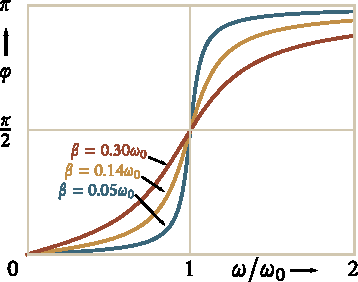
\includegraphics[scale=0.95]{figures/ch_07/fig_7_25.pdf}
		\caption[]{}
		\label{fig:7_25}
	\end{center}
	\vspace{-0.8cm}
\end{figure}

Từ hình \fig{7_22} rõ ràng là dao động cưỡng bức chậm pha so với lực cưỡng bức thêm vào đó độ lớn của độ chậm $\varphi$ nằm trong phạm vi từ $0$ đến $\pi$. Sự phụ thuộc của $\varphi$ vào $\omega$ với các giá trị khác nhau của $\beta$ được trình bày bằng đồ thị trên hình \fig{7_25}. Tần số $\omega_0$ ứng với $\varphi=\pi/2$. Tần số cộng hưởng nhỏ hơn tần số riêng [xem \eqn{7_127}]. Do đó, lúc cộng hưởng $\varphi<\pi/2$. Với sự tắt dần yếu $\omega_{\text{c}}\approx\omega_0$ và có thể coi giá trị của $\varphi$ khi cộng hưởng bằng $\pi/2$.

Cần phải tính đến hiện tượng cộng hưởng khi thiết kế máy và các công trình loại khác nhau. Tần số dao động riêng của các thiết bị này không bao giờ được gần với tần số của các tác động khả dĩ bên ngoài. Chẳng hạn, tần số riêng của các rung động của thân tàu thủy hoặc của các cánh máy bay phải khác xa tần số dao động có thể do sự quay của chân vịt hoặc của cánh quạt gây ra. Trong trường hợp ngược lại các rung động có thể gây ra tai biến sẽ xuất hiện. Người ta đã biết các trường hợp mà các cầu đã bị sập đổ khi một đoàn quân đi đều bước qua cầu. Điều này xảy ra vì tần số dao động riêng của cầu gần với tần số mà đoàn quân đã đi đều bước.

Đồng thời hiện tượng cộng hưởng cũng thường rất có lợi, đặc biệt là trong âm học và trong kỹ thuật vô tuyến điện, v.v...

\section{Cộng hưởng tham số}\label{sec:7_13}

Trong trường hợp đã được xét ở mục trước lực cưỡng bức được đặt từ bên ngoài trực tiếp gây ra sự dời của hệ khỏi vị trí cân bằng. Còn có một dạng tác động khác từ ngoài mà nhờ đó có thể làm hệ đu đưa mạnh. Dạng tác động này là ở chỗ sự biến đổi tuần hoàn của một tham số nào đó của hệ được thực hiện cùng nhịp với các dao động, do đó chính hiện tượng này được gọi là \textbf{sự cộng hưởng tham số}.

\begin{figure}[!htb]
	\begin{center}
		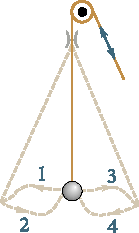
\includegraphics[scale=0.95]{figures/ch_07/fig_7_26.pdf}
		\caption[]{}
		\label{fig:7_26}
	\end{center}
\end{figure}

Để ví dụ ta lấy con lắc đơn giản nhất, đó là hòn bi treo trên sợi dây. Nếu làm biến đổi độ dài $l$ của con lắc một cách tuần hoàn bằng cách làm tăng nó tại lúc mà con lắc ở các vị trí biên và làm giảm tại lúc mà con lắc ở vị trí cân bằng (\fig{7_26}), thì con lắc bị đu đưa mạnh. Khi đó sự tăng năng lượng của con lắc xảy ra do công mà lực tác dụng lên sợi dây thực hiện. Lực căng của sợi dây khi con lắc dao động bị thay đổi: nó nhỏ hơn tại các vị trí biên khi vận tốc triệt tiêu và lớn hơn tại vị trí cân bằng khi vận tốc của con lắc là cực đại. Do đó khi con lắc được kéo dài ra, thì công âm của ngoại lực, về độ lớn, nhỏ hơn công dương được thực hiện khi con lắc được co ngắn lại. Rút cục, công của ngoại lực trong một chu kỳ là lớn hơn không.
